% -*- latex -*-

%\documentclass[pdf,ps2pdf,12pt,report,strict]{SANDreport}
\documentclass[12pt,report,strict]{SANDreport}
\usepackage{pslatex}
\usepackage[fancyhdr]{latex2man}
\usepackage{ifthen}
\usepackage{xspace}
\usepackage{relsize}
\usepackage{fancyvrb}

%%% % Comment this if not a draft.
%%% \usepackage[all,light]{draftcopy}

\usepackage{color}
\definecolor{yellow}{rgb}{1,1,0}
\definecolor{black}{rgb}{0,0,0}
\definecolor{ltcyan}{rgb}{.75,1,1}
\definecolor{red}{rgb}{1,0,0}

% This wonderful package allows hyphenation in tt fonts and hyphenation of
% words with underscores in them.
\usepackage[htt]{hyphenat}

\usepackage{makeidx}
\makeindex

\usepackage{hyperref}
\hypersetup{pdftitle={@TITLE@}}
\hypersetup{pdfauthor={Kenneth Moreland}}
% \hypersetup{colorlinks}
% \hypersetup{linkcolor=blue}
% \hypersetup{linkcolor=blue}
\hypersetup{breaklinks}
\hypersetup{pagebackref}
\hypersetup{pdfstartpage=3}

% -----------------------------------------------------------------------------
%
% Set the title, author, and date
%

\title{@TITLE@ \\
  \relsize{-2}Version @VERSION@
}
\author{Kenneth~Moreland \\
  Data Analysis and Visualization \\
  Sandia National Laboratories \\
  P.O. Box 5800  MS 1323 \\
  Albuquerque, NM  87185-1323 \\
  kmorel@sandia.gov
}

% There is a "Printed" date on the title page of a SAND report, so
% the generic \date should generally be empty.
\date{}

% -----------------------------------------------------------------------------
% Set some things we need for SAND reports. These are mandatory
%
\SANDnum{SAND2010-7451}
\SANDprintDate{November 2010}
\SANDauthor{Kenneth~Moreland}

% -----------------------------------------------------------------------------
% Include the markings required for the SAND report.  These are actually
% the default and not strictly necessary.
\SANDreleaseType{Unlimited Release}
\SANDmarkCover{Approved for public release; further dissemination unlimited.}

%-----------------------------------------------------------------------------
% The following definition does not have a default value and will not
% print anything, if not defined
\SANDsupersed{SAND2009-3170}{May 2009}

%-----------------------------------------------------------------------------
% Commands for inserting common words.
\newcommand{\IceT}{IceT\xspace}
\newcommand{\OpenGL}{\index{OpenGL}OpenGL\xspace}
\newcommand{\MPI}{\index{MPI}{MPI}\xspace}

% Commands for words with special meanings.
\newcommand*{\keyterm}[1]{\textbf{#1}}

\newcommand{\sticky}[1]{{\color{red}\textsc{[#1]}}}

\CustomVerbatimEnvironment{code}{Verbatim}{fontsize=\small}
\newcommand*{\codeinput}[2][]{%
  \VerbatimInput[fontsize=\small,#1]{#2}%
}

% A special section for man pages.  We don't really want these to show up
% in the table of contents.
% \newcommand{\mansection}[1]{
%   \\[\baselineskip]
%   \textbf{\textsc{\large #1}} \\[0.5\baselineskip]
% }
\makeatletter
\renewcommand{\subsection}{\@startsection
  {subsection}
  {2}
  {0mm}
  {-\baselineskip}
  {0.5\baselineskip}
  {\normalfont\large\bfseries\scshape}
}
\makeatother
\newcommand*{\mansection}[1]{\subsection*{#1}}  

% The latex2man Name environment does not mesh well with the SAND
% environment, nor is it designed to have several man pages in the same
% document.  Thus, we change it to fit.
\newcommand*{\currentmansection}{none}
\renewenvironment{Name}[5]{
  % #1 Man Chapter
  % #2 Name
  % #3 Author
  % #4 Tool
  % #5 Title
  \clearpage
  \renewcommand{\currentmansection}{#2}
  \index{\currentmansection|(textbf}
  \lhead[#2]{}
  \rhead[]{#2}
  \phantomsection
  \addcontentsline{toc}{section}{\currentmansection}
  \label{manpage:#2}
  \mansection{Name}
  #5
}{
  \index{\currentmansection|)}
}

% Change the latex2man Table environment.  Mostly to get rid of the
% indentation it places on the left hand side.  The nopagebreak option
% tries to avoid adding a page break (which can add a lot of space on the
% previous page).  The raggedbottom option says that if a page break is
% absolutely necessary, do not try to make the bottom of the previous page
% to the bottom of the page; it will add a bunch of space in the middle
% that will look bad.  The flush bottom option restores normal page flush
% operation.
\newlength{\tableindent}
\settowidth{\tableindent}{\enspace}
\addtolength{\tableindent}{\parindent}
\renewenvironment{Table}[1]{%
  \raggedbottom%
  \par\hspace*{-\tableindent}%
  \begin{tabular}{*{#1}{l}}%
}{%
  \end{tabular}%
  \nopagebreak[3]%
  \flushbottom%
  \par%
}

% Commands for typesetting C identifiers.
\newcommand{\textC}[1]{\texttt{#1}}                     % Basic C code.
\newcommand{\textCF}[1]{\textbf{\textC{#1}}}
\newcommand{\textCT}[1]{\textbf{\textC{#1}}}

\newcommand{\CType}[1]{\index{#1}\textCT{#1}}           % A documented type.
\newcommand{\CFunc}[2][!*!]{%                           % A documented function.
  % Only reference if not in that man section.
  \ifthenelse%
      {\equal{#1}{!*!}}%
      {\ifthenelse%
        {\equal{#2}{\currentmansection}}%
        {\textCF{#2}}%
        {\index{#2}\hyperref[manpage:#2]{\textCF{#2}}}%
      }%
      {\ifthenelse%
        {\equal{#1}{\currentmansection}}%
        {\textCF{#2}}%
        {\index{#1}\hyperref[manpage:#1]{\textCF{#2}}}%
      }%
}
\newcommand*{\CFuncExternal}[1]{%                       % An external function.
  \index{#1}%
  \textCF{#1}%
}
\newcommand*{\CFuncSeeAlso}[1]{%                        % A see also reference.
  \hyperref[manpage:#1]{\textCF{#1}}%
}
\newcommand*{\CTypeExternal}[1]{\CType{#1}}             % An external type.

\newcommand*{\CArg}[1]{\emph{\textC{#1}}}               % A function argument.
\newcommand*{\CEnum}[1]{\index{#1}\textbf{\textC{#1}}}  % A const enumeration.
\newcommand*{\CErrorEnum}[1]{\textbf{\textC{#1}}}       % An error constant.

% Functions that have aliases for cross referencing and indexing.
\newcommand{\icetBoundingBoxf}{\CFunc[icetBoundingBox]{icetBoundingBoxf}\xspace}
\newcommand{\icetBoundingBoxd}{\CFunc[icetBoundingBox]{icetBoundingBoxd}\xspace}

\newcommand{\icetEnable}{\CFunc[icetEnable]{icetEnable}\xspace}
\newcommand{\icetDisable}{\CFunc[icetEnable]{icetDisable}\xspace}

\newcommand{\icetGetBitFieldv}{\CFunc[icetGet]{icetGetBitFieldv}\xspace}
\newcommand{\icetGetBooleanv}{\CFunc[icetGet]{icetGetBooleanv}\xspace}
\newcommand{\icetGetDoublev}{\CFunc[icetGet]{icetGetDoublev}\xspace}
\newcommand{\icetGetEnumv}{\CFunc[icetGet]{icetGetEnumv}\xspace}
\newcommand{\icetGetFloatv}{\CFunc[icetGet]{icetGetFloatv}\xspace}
\newcommand{\icetGetIntegerv}{\CFunc[icetGet]{icetGetIntegerv}\xspace}
\newcommand{\icetGetPointerv}{\CFunc[icetGet]{icetGetPointerv}\xspace}

\newcommand{\icetSetColorFormat}{\CFunc{icetSetColorFormat}\xspace}
\newcommand{\icetSetDepthFormat}{%
  \ifthenelse%
    {\equal{\currentmansection}{icetSetColorFormat}}%
    {\CFunc[icetSetColorFormat]{icetSetDepthFormat}}%
    {\CFunc{icetSetDepthFormat}}%
    \xspace%
}

\newcommand{\icetImageGetColorFormat}{\CFunc{icetImageGetColorFormat}\xspace}
\newcommand{\icetImageGetDepthFormat}{%
  \ifthenelse%
    {\equal{\currentmansection}{icetImageGetColorFormat}}%
    {\CFunc[icetImageGetColorFormat]{icetImageGetDepthFormat}}%
    {\CFunc{icetImageGetDepthFormat}}%
    \xspace%
}

\newcommand{\icetImageGetNumPixels}{\CFunc{icetImageGetNumPixels}\xspace}
\newcommand{\icetImageGetWidth}{%
  \ifthenelse%
    {\equal{\currentmansection}{icetImageGetNumPixels}}%
    {\CFunc[icetImageGetNumPixels]{icetImageGetWidth}}%
    {\CFunc{icetImageGetWidth}}%
    \xspace%
}
\newcommand{\icetImageGetHeight}{%
  \ifthenelse%
    {\equal{\currentmansection}{icetImageGetNumPixels}}%
    {\CFunc[icetImageGetNumPixels]{icetImageGetHeight}}%
    {\CFunc{icetImageGetHeight}}%
    \xspace%
}

\newcommand{\icetImageGetColor}{\CFunc{icetImageGetColor}\xspace}
\newcommand{\icetImageGetColorub}{\CFunc[icetImageGetColor]{icetImageGetColorub}\xspace}
\newcommand{\icetImageGetColorui}{\CFunc[icetImageGetColor]{icetImageGetColorui}\xspace}
\newcommand{\icetImageGetColorf}{\CFunc[icetImageGetColor]{icetImageGetColorf}\xspace}
\newcommand{\icetImageGetColorcub}{\CFunc[icetImageGetColor]{icetImageGetColorcub}\xspace}
\newcommand{\icetImageGetColorcui}{\CFunc[icetImageGetColor]{icetImageGetColorcui}\xspace}
\newcommand{\icetImageGetColorcf}{\CFunc[icetImageGetColor]{icetImageGetColorcf}\xspace}

\newcommand{\icetImageGetDepth}{%
  \ifthenelse%
    {\equal{\currentmansection}{icetImageGetColor}}%
    {\CFunc[icetImageGetColor]{icetImageGetDepth}}%
    {\CFunc{icetImageGetDepth}}%
    \xspace%
}
\newcommand{\icetImageGetDepthf}{%
  \ifthenelse%
    {\equal{\currentmansection}{icetImageGetColor}}%
    {\CFunc[icetImageGetColor]{icetImageGetDepthf}}%
    {\CFunc[icetImageGetDepth]{icetImageGetDepthf}}%
    \xspace%
}
\newcommand{\icetImageGetDepthcf}{%
  \ifthenelse%
    {\equal{\currentmansection}{icetImageGetColor}}%
    {\CFunc[icetImageGetColor]{icetImageGetDepthcf}}%
    {\CFunc[icetImageGetDepth]{icetImageGetDepthcf}}%
    \xspace%
}

\newcommand{\icetImageCopyColor}{\CFunc{icetImageCopyColor}\xspace}
\newcommand{\icetImageCopyColorub}{\CFunc[icetImageCopyColor]{icetImageCopyColorub}\xspace}
\newcommand{\icetImageCopyColorf}{\CFunc[icetImageCopyColor]{icetImageCopyColorf}\xspace}

\newcommand{\icetImageCopyDepth}{%
  \ifthenelse%
    {\equal{\currentmansection}{icetImageCopyColor}}%
    {\CFunc[icetImageCopyColor]{icetImageCopyDepth}}%
    {\CFunc{icetImageCopyDepth}}%
    \xspace%
}
\newcommand{\icetImageCopyDepthf}{%
  \ifthenelse%
    {\equal{\currentmansection}{icetImageCopyColor}}%
    {\CFunc[icetImageCopyColor]{icetImageCopyDepthf}}%
    {\CFunc[icetImageCopyDepth]{icetImageCopyDepthf}}%
    \xspace%
}

\newcommand{\icetUnsafeStateGetDouble}{%
  \CFunc[icetUnsafeStateGet]{icetUnsafeStateGetDouble}\xspace%
}
\newcommand{\icetUnsafeStateGetFloat}{%
  \CFunc[icetUnsafeStateGet]{icetUnsafeStateGetFloat}\xspace%
}
\newcommand{\icetUnsafeStateGetInteger}{%
  \CFunc[icetUnsafeStateGet]{icetUnsafeStateGetInteger}\xspace%
}
\newcommand{\icetUnsafeStateGetBoolean}{%
  \CFunc[icetUnsafeStateGet]{icetUnsafeStateGetBoolean}\xspace%
}
\newcommand{\icetUnsafeStateGetPointer}{%
  \CFunc[icetUnsafeStateGet]{icetUnsafeStateGetPointer}\xspace%
}

% Avoid putting figures on their own page.
\renewcommand{\textfraction}{0.05}
\renewcommand{\topfraction}{0.95}

% Make sure this is big enough so that only big figures end up on their own
% page but small enough so that if a figure does have to be on its own
% page, it won't push everything to the bottom because it's not big enough
% to have its own page.
\renewcommand{\floatpagefraction}{.75}

%-----------------------------------------------------------------------------
% The actual document.

\begin{document}

\sloppy
\maketitle

% An abstract is required for SAND reports.

\begin{abstract}
  The Image Composition Engine for Tiles (\IceT) is a high-performance
  sort-last parallel rendering library.  In addition to providing
  accelerated rendering for a standard display, \IceT provides the unique
  ability to generate images for tiled displays.  The overall resolution of
  the display may be several times larger than any viewport that may be
  rendered by a single machine.  This document is an overview of the user
  interface to \IceT.
\end{abstract}

%-----------------------------------------------------------------------------
% In case we every need an acknowledgement section.
\clearpage
\chapter*{Acknowledgement}

I would like to thank Brian Wylie.  It was his ``big ideas'' that got the
ball rolling on the \IceT algorithms and library, and it was his continuing
vision that pushed us on this path to parallel rendering.

I would also like to thank the folks at Kitware, Inc. for adopting the
\IceT library as the parallel rendering library for ParaView.  They also
maintain the \IceT code repository.  Without them, \IceT would probably be
collecting dust on a crashed RAID somewhere.

% -----------------------------------------------------------------------------
% The table of contents and list of figures and tables
% Comment out \listoffigures and \listoftables if there are no
% figures or tables. Make sure this starts on an odd numbered page
\cleardoublepage                % TOC needs to start on an odd page
\tableofcontents
\listoffigures
% \listoftables

% -----------------------------------------------------------------------------
% This is where the body of the report begins.
\SANDmain       % Start the main part of the report.

% -*- latex -*-


\chapter{Introduction}
\label{chap:Introduction}

The Image Composition Engine for Tiles (\IceT) is an API designed to enable
OpenGL applications to perform Sort-Last parallel rendering on very large
displays.  The displays are assumed to be tile displays.  The overall
resolution of the display may be several times larger than any viewport
that may be rendered by a single machine.  It is also assumed that several
processes in the parallel application are
\index{display~process}\keyterm{display processes}.  That is, their entire
display window makes up part of the display.

The design philosophy behind \IceT is to allow very large sets of polygons
to be displayed on very high resolution displays.  As such, fast frame
rates are sacrificed in lieu of very scalable and very high polygon/second
rendering rates.  That said, there are many features in \IceT that allow an
application to achieve interactive rates.  These include image inflation,
floating viewports, active pixel encoding, and data replication.  Together,
these features make \IceT a versatile parallel rendering application that
provides near optimal parallel rendering under most data size and image
size combinations.  As an example, the ParaView
application\footnote{\href{http://www.paraview.org}{http://www.paraview.org}}
is using \IceT for all of its parallel rendering needs ranging from a
desktop sized image to the world's largest tile displays and from polygon
counts ranging from 1 to 1 million (and growing).

\IceT is designed to take advantage of
\index{spatial~decomposition}\keyterm{spatial decomposition} of the
geometry being rendered.  That is, it works best if all the geometry on
each process is located in as small a region of space as possible.  When
this is true, each process usually projects geometry on only a small
section of the screen.  This results in less work for the compositing
engine.  This is of particular importance for displays with a large number
of pixels.

\IceT can also be used to perform sort-last parallel rendering to a single
display.  Such \index{single-tile~rendering}\keyterm{single-tile rendering}
is simply a special case of the multi-tile display \IceT was designed for.
Many of the optimizations done by \IceT apply to the single-tile mode.
Using \IceT for this purpose is quite worthwhile.  \IceT's performance
should rival that of other such software image compositors.

The rest of this document describes the use of the
\IceT
API.  There are also separate manual pages for each of the functions
described here.  For more details on
\IceT's
algorithms, see:

\begin{quote}
  Moreland, Wylie, and Pavlakos.  ``Sort-last parallel rendering for
  viewing extremely large data sets on tile displays,'' In
  \emph{Proceedings of IEEE Symposium on Parallel and Large-Data
    Visualization and Graphics}, October 2001, pp. 85--154.
\end{quote}


% -*- latex -*-

\chapter{Tutorial}
\label{chap:Tutorial}

In this chapter we outline the steps required to create a simple \IceT
application from building the \IceT source, using the created libraries,
and writing your own applications.  \IceT is solely responsible for the
image composition part of parallel rendering.  Thus, it relies on two other
APIs: \index{OpenGL}\keyterm{OpenGL} for rendering and a communication
layer for passing messages such as \index{MPI}\keyterm{MPI}, the Message
Passing Interface.  Both have implementations in nearly every computer
architecture.

This tutorial assumes the reader is familiar with OpenGL.  If this is your
first experience with OpenGL programing, consider trying some typical
serial rendering before jumping into the parallel rendering domain.  A
familiarity with MPI is also helpful.

\section{Building \IceT}
\label{sec:Tutorial:Building_IceT}

The \IceT build process is very portable.  It can be compiled on Microsoft
Windows, Macintosh OS X, and a wide variety of Unix implementations.  \IceT
can be built on just about any platform that has an
\index{OpenGL}OpenGL~1.1 compliant installation.  Most modern operating
systems come distributed with OpenGL.  For those that are not, you can
usually use the \index{Mesa~3D}\keyterm{Mesa 3D} library
(\href{www.mesa3d.org}{www.mesa3d.org}), a software implementation of
OpenGL.  An installation of MPI is also almost always needed, although not
strictly required.  \index{MPICH}\keyterm{MPICH}
(\href{http://www-unix.mcs.anl.gov/mpi/mpich2/}{http://www-unix.mcs.anl.gov/mpi/mpich2/})
is a free and widely portable implementation of MPI.

\IceT uses \index{CMake}\keyterm{CMake} to build across so many different
platforms.  As such, you will have to download the CMake build tools from
\href{www.cmake.org}{www.cmake.org} and install.  Then, create a build
directory and run the CMake program (from the ``Start'' menu on Windows or
ccmake on Unix and Mac OS X).  CMake will determine the parameters of your
system and do its best to find libraries on which \IceT depends.  The CMake
program, shown in Figure~\ref{fig:Tutorial:ccmake} will also provide a GUI
to allow you to easily change build parameters and external libraries.
\begin{figure}
  \centering
  \includegraphics[height=1.5in]{images/ccmakeUnix}
  \qquad
  \includegraphics[height=1.5in]{images/ccmakeWindows}
  \caption[CMake user interface.]{The CMake user interface.  The Unix
    version is on the left whereas the Microsoft Windows version is on the
    right.}
  \label{fig:Tutorial:ccmake}
\end{figure}

CMake will generate a set of build files for the local system.  The type of
files depends on the type of machine you are using and the compile system
you have chosen to use.  On Unix machines, make files are the most common.
On Windows, you usually generate MSVC project files or nmake files.  On Mac
OS X, either make files or Xcode project files are commonly generated based
on user selection.  You then use the native build system to build and,
optionally, install \IceT.

\section{Linking to \IceT Libraries}
\label{sec:Tutorial:Linking_to_IceT_Libraries}

\IceT comes with three libraries: \index{icet (library)}\keyterm{icet},
\index{icet\_strategies~(library)}\keyterm{icet\_strategies}, and
\index{icet\_mpi~(library)}\keyterm{icet\_mpi}.  The actual filenames of
these libraries varies depending on the filesystem and build type.  For
example, on most Unix systems, a static build results in filenames of
\index{libicet.a}libicet.a and the like whereas shared libraries are
libicet.so.  Windows has libraries with names like icet.lib as well as
icet.dll if building shared libraries.  However, the difference in these
filenames usually hidden by the build system, especially if you use a
portable build system like \index{CMake}CMake.

You are, of course, free to use whatever build system you like, whether it
be system specific or cross platform.  Using \IceT is simply a matter of
finding the header and library files.  However, because \IceT is built with
CMake, it comes with some extra facilities for helping other CMake builds
find it.  This section will give you the bare minimum you need to set up
CMake to build an application using \IceT.  Readers interested more about
CMake should pick up a copy of \emph{Mastering CMake} by Ken Martin and
Bill Hoffman.

You define a build system with CMake by creating a
\index{CMakeLists.txt}\keyterm{CMakeLists.txt} file.  The CMakeLists.txt
file is basically a simple script that gives commands the CMake to tell it
how to build your project.  Most CMakeLists.txt files start with the
\textC{PROJECT} command, which associates a name with your project and
optionally specifies a language.
\begin{code}
PROJECT(IceT_Tutorial)
\end{code}

Distributed with the \IceT source code is a file called
\index{FindIceT.cmake}\keyterm{FindIceT.cmake} that provides all the CMake
facilities needed to find and use an \IceT build.  It works by finding a
file called \index{ICETConfig.cmake}\keyterm{ICETConfig.cmake}, which is
written when \IceT is built and contains all the necessary build settings.
The FindIceT.cmake script can be invoked with the \textC{FIND\_PACKAGE}
command.  After the \IceT package is found, a variable named
\textC{ICET\_USE\_FILE} is set to a file that may be \textC{INCLUDE}d in
your project to point it to the directories containing the header and
library files.
\begin{code}
FIND_PACKAGE(IceT REQUIRED)
INCLUDE(${ICET_USE_FILE})
\end{code}
%$

Any application using \IceT will also be using \index{OpenGL}OpenGL and
almost all will be using \index{MPI}MPI.  In addition, the example in the
following section also uses \index{GLUT}GLUT for window management.  CMake
comes with modules to find all three of these libraries, which makes it
easy to include in our project.
\begin{code}
FIND_PACKAGE(OpenGL REQUIRED)
FIND_PACKAGE(GLUT REQUIRED)
FIND_PACKAGE(MPI REQUIRED)

MARK_AS_ADVANCED(CLEAR
  MPI_INCLUDE_PATH
  MPI_LIBRARY
  MPI_EXTRA_LIBRARY
  )

INCLUDE_DIRECTORIES(
  ${OPENGL_INCLUDE_DIR}
  ${MPI_INCLUDE_PATH}
  ${GLUT_INCLUDE_DIR}
  )
\end{code}
%$

The only think left to do is to tell CMake to build a program from a set of
sources and libraries specified with the \textC{ADD\_EXECUTABLE} and
\textC{TARGET\_LINK\_LIBRARIES} commands, respectively.
\begin{code}
ADD_EXECUTABLE(Tutorial Tutorial.c)
TARGET_LINK_LIBRARIES(Tutorial
  ${OPENGL_LIBRARIES}
  ${GLUT_LIBRARIES}
  ${MPI_LIBRARY}
  ${MPI_EXTRA_LIBRARY}
  ${ICET_CORE_LIBS}
  ${ICET_MPI_LIBS}
  )
\end{code}

\section{Creating \IceT Enabled Applications}
\label{sec:Tutorial:Creating_IceT_Enabled_Applications}

To use \IceT, include it's header:
\index{ice-t.h}\index{GL/ice-t.h}\textC{GL/ice-t.h}.  You will almost
always need to also include the header containing an MPI version of an
\IceT communicator:
\index{ice-t\_mpi.h}\index{GL/ice-t\_mpi.h}\textC{GL/ice-t\_mpi.h}.  On the
rare occasion that you need to use \IceT with a communication layer other
than MPI, you can define a custom communicator as described in
Chapter~\ref{chap:Communicators}.
\begin{code}
#include <GL/ice-t.h>
#include <GL/ice-t_mpi.h>
\end{code}

Before you call any \IceT functions, you need to initialize MPI by calling
\textC{MPI\_Init}\index{MPI\_Init}.  You will also need to create an OpenGL
context (that is, open an OpenGL window).  Do this by first creating an
\IceT \index{communicator}\keyterm{communicator} from an MPI communicator
and then using that to create an
\index{context!\IceT}{\keyterm{\IceT context}.
\index{icetCreateMPICommunicator}
\index{icetCreateContext}
\begin{code}
    comm = icetCreateMPICommunicator(MPI_COMM_WORLD);
    context = icetCreateContext(comm);
\end{code}
In the proceeding code, \textC{comm} is of type
\index{IceTCommunicator}\textC{IceTCommunicator} and \textC{context} is of
type \index{IceTContext}\textC{IceTContext}.

Now that we have created and activated an \IceT communicator, as well as
initialized the \IceT \index{state}\keyterm{state}, we can start using
\IceT.  It is often useful to first query \IceT on the size of the parallel
job it is running in and what is the local process id, or
\index{rank}\keyterm{rank}.  The values are stored in variables of type
\textC{GLint}.
\begin{code}
    icetGetIntegerv(ICET_RANK, &rank);
    icetGetIntegerv(ICET_NUM_PROCESSES, &num_proc);
\end{code}

In addition to an \IceT context, you will also need an
\index{context!\OpenGL}\keyterm{\OpenGL context}.  In other words, you need
to make the rendering window in which the \OpenGL rendering commands will
go.  The process for doing this is greatly dependent on the windowing
system and beyond the scope of this document.  It is usually easiest to use
a third party API to do this.  If you are not already using a GUI tool that
generates \OpenGL windows for you, then the \index{GLUT}\keyterm{GLUT} API
is a popular choice for simple applications.

Before rendering, we need to tell \IceT the layout of the tile display
using the \CFunc{icetResetTiles} and \CFunc{icetAddTile} functions.  These
commands must be executed with the same arguments on all processes of the
parallel job.  \IceT will assume that you setup the same display layout
everywhere.

If you are not actually driving a tile display and instead just generating
a desktop-sized image, the following commands will correctly establish the
\IceT state.
\begin{code}
    icetResetTiles();
    icetAddTile(0, 0, WINDOW_WIDTH, WINDOW_HEIGHT, 0);
\end{code}

The \CFunc{icetResetTiles} function simply tells \IceT that you are about
to define a display layout.  Each call to \CFunc{icetAddTile} defines a
tile in the display.  In the case of a single image, the
\index{single-tile~rendering}\keyterm{single-tile rendering} mode,
\CFunc{icetAddTile} is called only once.  The first two arguments to
\CFunc{icetAddTile} have no effect in this mode.  The third and fourth
arguments are the width and height of the image to create.  Usually you set
this to the width and the height of the display window, but the
\hyperref[sec:Customizing_Compositing:Image_Inflation]{Image Inflation}
section in Chapter~\ref{chap:Customizing_Compositing} describes other usage
for these parameters.  The final argument is the rank of the
\index{display~process}\keyterm{display process}.  After a rendering the
final complete image will available only on this process.  In the example
above, we have direct the image to go to process zero, often referred to as
the \index{root~process}\keyterm{root process}.

To define an actual tile display, simply call the \CFunc{icetAddTile}
function multiple times.  When describing tiles in a display, the first two
arguments of \CFunc{icetAddTile} describe where the lower left corner of
the tile is located in respect to the overall display.  All together, the
first four arguments specify a viewport for the tile in an a single,
cohesive high resolution display (which is what we are trying to achieve
with our tile display).  The code below defines a $2 \times 2$ tile display
with the top two tiles displayed by processes 0 and 1 and the bottom two
tiles displayed by processes 2 and 3.
\begin{code}
    icetResetTiles();
    icetAddTile(0,           WINDOW_HEIGHT, WINDOW_WIDTH, WINDOW_HEIGHT, 0);
    icetAddTile(WINDOW_WIDTH,WINDOW_HEIGHT, WINDOW_WIDTH, WINDOW_HEIGHT, 1);
    icetAddTile(0,           0,             WINDOW_WIDTH, WINDOW_HEIGHT, 2);
    icetAddTile(WINDOW_WIDTH,0,             WINDOW_WIDTH, WINDOW_HEIGHT, 3);
\end{code}

\IceT contains several \index{strategy}\keyterm{strategies} for image
composition.  Changing the strategy modifies the algorithm \IceT uses for
parallel image compositing.  You need to tell \IceT which strategy to use
with the \CFunc{icetStrategy} function.  The code below sets \IceT to use
the \index{strategy!reduce}\keyterm{reduce strategy}, which has proven to
be an all-around good performer.
\begin{code}
    icetStrategy(ICET_STRATEGY_REDUCE);
\end{code}
Like with the display set up, all processes must set the same strategy.

\IceT is almost ready to go.  We just need to tell it some minimal
information about how to render your geometry.  First, \IceT needs to know
the spatial extent of the geometry to be drawn (in object space).  The most
natural way to do this is to use the \CFunc{icetBoundingBox} function,
which defines an axis-aligned box defined by the minimum and maximum
coordinates in each dimension.
\begin{code}
    icetBoundingBoxf(x_min, x_max, y_min, y_max, z_min, z_max);
\end{code}
The parameters can, and should be, different on each process, since each
process will have a different partition of data.  Strictly speaking,
identifying the geometry bounds is not necessary.  If they are not defined,
\IceT will assume the geometry covers the entire screen.  When rendering a
single small image, the information is of little consequence.  However,
when rendering larger images this information can dramatically improve the
performance of image composting.  Specifying the bounds can be critical on
large tile displays.

The second and final piece of information \IceT needs is a way to draw your
geometry.  \IceT achieves this through a
\index{drawing~callback}\index{callback|see{drawing~callback}}\index{rendering~callback|see{drawing~callback}}\keyterm{drawing
  callback}.
\begin{code}
    icetDrawFunc(drawScene);
\end{code}
The drawing callback is a pointer to any function that issues
\OpenGL commands that render geometry to the active frame buffer.  The
callback is free to issue most \OpenGL so long as it restores all the
\OpenGL state (except, of course, frame buffer contents).  Also, the
callback function should modify neither the projection matrix nor the
clear color.  Care needs to be taken if the callback modifies the model view
matrix.  More details are given in the
\hyperref[sec:Basic_Usage::Drawing_Callback]{Drawing Callback} section of
Chapter~\ref{chap:Basic_Usage}.

\IceT is now ready to render.  Rendering is initiated with a call to
\CFunc{icetDrawFrame}.  The \CFunc{icetDrawFrame} must be called on all
processes.  The function will render the scene using the provided
\index{drawing~callback}drawing callback, composite the image, and place
the appropriate images in the back \OpenGL buffers of the appropriate
\index{display~process}display processes.
\begin{code}
    icetDrawFrame();
\end{code}

Parallel rendering is now enabled in your application.  Simply call
\CFunc{icetDrawFrame} every time you wish to draw a new image.  The
geometry rendered by your \index{drawing~callback} may change from frame to
frame so long as you ensure that you also update \IceT with the bounds of
your geometry if it changes.

The following code is a full example of a simple \IceT application.  Do not
be alarmed by the length.  The majority of the code is spent in setting up
the supporting libraries (OpenGL, GLUT, and MPI) and in comments.

\codeinput{examples/Tutorial.c}


% -*- latex -*-

\chapter{Basic Usage}
\label{chap:Basic_Usage}

In this chapter we describe in greater detail the basic features of \IceT.
The tutorial given in Chapter~\ref{chap:Tutorial} is a good place to
start building your applications.  You can then consult this chapter and
later ones for more details on the operations as well as descriptions of
further features.

Prototypes for the majority of \IceT types, functions, and identifiers can
be found in the \index{IceT.h}\textC{IceT.h} header file.  If you are using
\OpenGL for rendering, which is common, you will probably want to include
the header \index{IceTGL.h}\textC{IceTGL.h}.  You will also almost always
need to include the header \index{IceTMPI.h}\textC{IceTMPI.h}.
Chapter~\ref{chap:Communicators} provides more details on this last
header file's function.
\begin{code}
#include <IceT.h>
#include <IceTGL.h>
#include <IceTMPI.h>
\end{code}

\section{The State Machine}
\label{sec:Basic_Usage:The_State_Machine}

\index{state|(}

The \IceT API borrows many concepts from \index{OpenGL}OpenGL.  One major
concept taken is that of a state machine.  At all times \IceT maintains a
current state.  The state can influence the operations that \IceT makes,
and \IceT's operations can modify the state.

\index{context!\IceT|(}
\IceT can manage multiple collections of state at the same time.  It does
this by associating each state with a
\keyterm{context}.  At any given time, there is at
most one active context.  Any \IceT function called works using the current
active context.

Contexts are created and destroyed with \CFunc{icetCreateContext} and
\CFunc{icetDestroyContext}, respectively.

\begin{Table}{3}
  \CType{IceTContext}\textC{ }\CFunc{icetCreateContext}\textC{(}&\CType{IceTCommunicator}&\CArg{comm}\quad\textC{);}
\end{Table}
\begin{Table}{3}
  \textC{void }\CFunc{icetDestroyContext}\textC{(}&\CType{IceTContext}&\CArg{context}\quad\textC{;}
\end{Table}

These functions work with an object of type \CType{IceTContext}.
\CType{IceTContext} is an opaque type; you are not meant to directly access
it.  Instead, you pass the object to functions to do the work for you.

The \CFunc{icetCreateContext} function requires an object of type
\CType{IceTCommunicator}.  This is another opaque type that is described in
more detail in Chapter~\ref{chap:Communicators}.  For now, just know that
you can create one from an MPI communicator using the
\CFunc{icetCreateMPICommunicator} function.

\begin{Table}{3}
  \CType{IceTCommunicator}\textC{ }\CFunc{icetCreateMPICommunicator}\textC{(} \\
  \qquad\qquad\qquad\qquad\qquad\qquad\qquad\qquad\qquad\qquad\qquad
  \CTypeExternal{MPI\_Comm}\quad\CArg{mpi\_comm}\quad\textC{);}
\end{Table}
\begin{Table}{3}
  \textC{void }\CFunc{icetDestroyMPICommunicator}\textC{(}&\CType{IceTCommunicator}&\CArg{comm}\quad\textC{);}
\end{Table}

Also be aware that if you plan to use \IceT's \OpenGL layer, you will need
to initialize it with \CFunc{icetGLInitialize}.  You can query whether the
\OpenGL layer has be initialized with \CFunc{icetGLIsInitialized}.

\begin{Table}{3}
  \textC{void }\CFunc{icetGLInitialize}\textC{(}&\textC{void}&\textC{);}
\end{Table}
\begin{Table}{3}
  \textC{IceTBoolean }\CFunc{icetGLIsInitialized}\textC{(}&\textC{void}&\textC{);}
\end{Table}

It is good practice to call \CFunc{icetGLInitialize} immediately after
creating a context with \CFunc{icetCreateContext} to always ensure that the
\OpenGL layer is ready to be used (assuming you plan to use it).

The following code gives the common boilerplate for setting up your initial
\IceT context.

\begin{code}
#include <IceT.h>
#include <IceTGL.h>
#include <IceTMPI.h>

int main(int argc, char **argv)
{
  IceTCommunicator icetComm;
  IceTContext icetContext;

  /* Setup MPI. */
  MPI_Init(&argc, &argv);

  /* Setup an IceT context.  If we are only creating one, this context will
   * always be current. */
  icetComm = icetCreateMPICommunicator(MPI_COMM_WORLD);
  icetContext = icetCreateContext(icetComm);
  icetDestroyMPICommunicator(icetComm);

  /* Initialize the OpenGL layer. */
  icetGLInitialize();

  /* Start your parallel rendering program here. */

  /* Cleanup IceT and MPI. */
  icetDestroyContext(icetContext);
  MPI_Finalize();

  return 0;
}
\end{code}

Any number of contexts may be created, each with its own associated state.
At any given time, a single given context is
\index{content!current}\keyterm{current}.  All \IceT operations are applied
with the state attached to the current context.  A handle to the current
\IceT context can be retrieved with the \CFunc{icetGetContext} function,
and he current context can be changed by using the \CFunc{icetSetContext}
function.

\begin{Table}{3}
  \CType{IceTContext}\textC{ }\CFunc{icetGetContext}\textC{(}&\textC{void}&\textC{);}
\end{Table}

\begin{Table}{3}
  \textC{void }\CFunc{icetSetContext}\textC{(}&\CType{IceTContext}&\CArg{context}\quad\textC{);}
\end{Table}

Changing the context is a fast and easy way to swap states.  This could be
used, for example, to switch between rendering modes.  One context could be
used for a full resolution image, and another could use
\index{image~inflation}\keyterm{image inflation} (described in
Chapter~\ref{sec:Customizing_Compositing:Image_Inflation}) to make faster
but coarser images during interaction.

When a context is created, its state is initialized to default values.  You
can effectively ``duplicate'' a context by copying the state of one context
to another using the \CFunc{icetCopyState} function.

\begin{Table}{3}
  \textC{void }\CFunc{icetCopyState}\textC{(}&\CType{IceTContext}&\CArg{dest}\textC{,} \\
  &\textC{const }\CType{IceTContext}&\CArg{src}\quad\textC{);}
\end{Table}

\index{context!\IceT|)}

The state of a context comprises a group of key/value pairs.  The state can
be queried by using any of the \CFunc{icetGet} functions.

\begin{Table}{3}
  \textC{void }\icetGetDoublev\textC{(}&\textC{IceTEnum}&\CArg{pname}\textC{,} \\
  &\textC{IceTDouble *}&\CArg{params}\quad\textC{);}
\end{Table}

\begin{Table}{3}
  \textC{void }\icetGetFloatv\textC{(}&\textC{IceTEnum}&\CArg{pname}\textC{,} \\
  &\textC{IceTFloat *}&\CArg{params}\quad\textC{);}
\end{Table}

\begin{Table}{3}
  \textC{void }\icetGetIntegerv\textC{(}&\textC{IceTEnum}&\CArg{pname}\textC{,} \\
  &\textC{IceTInt *}&\CArg{params}\quad\textC{);}
\end{Table}

\begin{Table}{3}
  \textC{void }\icetGetBooleanv\textC{(}&\textC{IceTEnum}&\CArg{pname}\textC{,} \\
  &\textC{IceTBoolean *}&\CArg{params}\quad\textC{);}
\end{Table}

\begin{Table}{3}
  \textC{void }\icetGetPointerv\textC{(}&\textC{IceTEnum}&\CArg{pname}\textC{,} \\
  &\textC{IceTVoid **}&\CArg{params}\quad\textC{);}
\end{Table}

The valid keys that can be used in the \CFunc{icetGet} functions are listed
in the \CFunc{icetGet} documentation starting on
page~\pageref{manpage:icetGet}.  There is no way to directly set these
state variables.  Instead, they are set either by \IceT configuration
functions or indirectly as part of the operation of \IceT.  The
documentation for \CFunc{icetGet} also describes which functions can be
used to set each state entry (assuming the user has control of that state
entry).

There is a special set of state entries that toggle \IceT options.  Although
you can query this state with the \icetGetBooleanv function, it is more
typical to use the \CFunc{icetIsEnabled} function.  Also unlike the other
state variables, these variables can be directly manipulated with the
\CFunc{icetEnable} and \CFunc{icetDisable} functions.

\begin{Table}{4}
  \textC{IceTBoolean }\CFunc{icetIsEnabled}\textC{(}&\textC{IceTEnum}&\CArg{pname}&\textC{);}
\end{Table}

\begin{Table}{4}
  \textC{void }\icetEnable&\textC{(}&\textC{IceTEnum}&\CArg{pname}\quad\textC{);}
\end{Table}

\begin{Table}{4}
  \textC{void }\icetDisable&\textC{(}&\textC{IceTEnum}&\CArg{pname}\quad\textC{);}
\end{Table}

The options queried with \CFunc{icetIsEnabled} and manipulated with
\CFunc{icetEnable} and \CFunc{icetDisable} are listed in the
\CFunc{icetEnable} documentation starting on
page~\pageref{manpage:icetEnable}.

\index{state|)}


\section{Diagnostics}
\label{sec:Basic_Usage:Diagnostics}

\index{diagnostics|(}

The \IceT library has a mechanism for reporting diagnostics.  There are
three levels of diagnostics.  \index{error}\keyterm{Errors} are anomalous
conditions that \IceT considers a critical failure.  An occurrence of an
error generally means that the future \IceT operations will have undefined
behavior.  When \IceT is compiled in debug mode, a seg fault is
intentionally raised when an error occurs to make it easier to attach a
debugger to the point where the error occurred.

\index{warning}\keyterm{Warnings} are detections of anomalous conditions
that are not as severe as errors.  When a warning occurs, the current
operation may produce the incorrect results, but future operations should
continue to work.

\IceT also can also provide a large volume of \index{debug}\keyterm{debug}
messages.  These messages simply indicate the status of \IceT operations as
they progress.  They are generally of no use to anyone who is not trying to
develop or debug \IceT operations.

\IceT diagnostics are controlled with the \CFunc{icetDiagnostics} function.

\begin{Table}{3}
  \textC{void }\CFunc{icetDiagnostics}\textC{(}&\textC{IceTBitField}&\CArg{mask}\quad\textC{);}
\end{Table}

The \CFunc{icetDiagnostics} function takes a set of flags that can me or-ed
together.  The diagnostics for errors, warnings, and debug statements can
be set by passing the \CEnum{ICET\_DIAG\_ERRORS},
\CEnum{ICET\_DIAG\_WARNINGS}, and \CEnum{ICET\_DIAG\_DEBUG} flags, respectively.
Turning on warnings implicitly turns on errors and turning on debug
statements implicitly turns on errors and warnings (although there is no
problem with redundantly specifying these flags).

\IceT has the ability to report diagnostics either on all processes or only
on the \index{root~process}\keyterm{root process} (the process with rank
0).  This behavior is controlled by the \CEnum{ICET\_DIAG\_ROOT\_NODE} and
\CEnum{ICET\_DIAG\_ALL\_NODES} flags.  Many diagnostic messages occur on
all nodes when they occur, so reporting only on node 0 can greatly reduce
the number of messages with which to contend.  However, messages can differ
between processes or may not occur on all processes.

The special flags \CEnum{ICET\_DIAG\_FULL} and \CEnum{ICET\_DIAG\_OFF} turn
all possible diagnostics on and all diagnostics completely off,
respectively.

By default, \IceT displays errors and warnings on all nodes.  You can get
the current diagnostic level by calling \CFunc{icetGet} with
\CEnum{ICET\_DIAGNOSTIC\_LEVEL}.

\index{diagnostics|)}


\section{Display Definition}
\label{sec:Basic_Usage:Display_Definition}

\index{display~definition|(}
\index{tile~definition|(}

\IceT assumes that the tiled display it is driving has each tile connected
to the graphics output of one of the processes in the parallel job in which
it is running.  This type of arrangement is natural for any tiled display
driven by a graphics cluster, and is the delivery method of many graphics
APIs. %\lcite{Buck00,Humphreys00,Humphreys02,Samanta99}

\IceT defines the configuration of a tiled display by using a
\index{logical~global~display}\index{global~display}\keyterm{logical global
  display} with an infinite \footnote{Well, OK.  The logical global display
  only stretches as far as the 32-bit numbers that are used to define
  viewports.  But that's still way bigger than any physical display that we
  can possibly conceive, so conceptually we call it infinite.} number of
pixels in both the horizontal and vertical directions.  The definition of
each tile comprises the identifier for the process connected to the
physical projection and the \index{viewport}\keyterm{viewport} (position
and size) of the tile in the global display.  \IceT implicitly defines the
rectangle that tightly encompasses all of the tile viewports as the
viewable area and snaps the viewing region (defined by the OpenGL viewing
matrices) to this area.

\begin{figure}
  \centering
  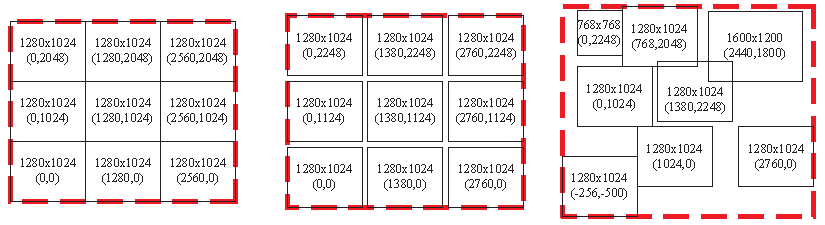
\includegraphics{images/ExampleTileConfig}
  \caption[Defining a tile display.]{Defining a tile display with viewports
    in a logical global display.  Three possible tile arrangements are
    shown.  The bounds of each tile is drawn with the viewport given
    inside.  The viewable area is shown with a dashed line.}
  \label{fig:BasicUsage:tile_layout}
\end{figure}

Figure~\ref{fig:BasicUsage:tile_layout} shows some possible tile
arrangements.  Mullions or overlaps of the tiles in the physical display
can be represented by the spacing or overlap of the viewports in the
logical display.  \IceT does not require the tile layout to have any
regularity.  Chaotic layouts like that shown in the right image of
Figure~\ref{fig:BasicUsage:tile_layout} are legal, although probably not
very useful.  It is allowed, and in fact encouraged, to have processes that
are not directly connected to the tiled display.  These
\index{non-display~process}\keyterm{non-display} processes still contribute
to the image compositing work and will reduce the overall time to render an
image.

The display is defined using the \CFunc{icetResetTiles} and
\CFunc{icetAddTile} functions.  Any previous tile definition is first
cleared out using \CFunc{icetResetTiles} and new tiles are added, one at a
time, using \CFunc{icetAddTile}.

\begin{Table}{3}
  \textC{void }\CFunc{icetResetTiles}\textC{(}&\textC{void}&\textC{)}
\end{Table}

\begin{Table}{3}
  \textC{int }\CFunc{icetAddTile}\textC{(}&\textC{IceTInt}&\CArg{x}\textC{,} \\
    &\textC{IceTInt}&\CArg{y}\textC{,} \\
    &\textC{IceTSizeType}&\CArg{width}\textC{,} \\
    &\textC{IceTSizeType}&\CArg{height}\textC{,} \\
    &\textC{int}&\CArg{display\_rank}\quad\textC{);}
\end{Table}

Each tile is specified using screen coordinates in the logical global
display: the position of the lower left corner and the width and height of
the tile.  Each tile also has a \index{display~process}\keyterm{display
  process} associated with it.  After an image is completely rendered and
composited, the screen section belonging to this tile will be placed in the
process at the given rank.

The following code demonstrates a common example for establishing the tile
layout: a grid of projectors.  The arrangement of projectors in this
example assume that the projectors are connected to processes in the order
of left to right and then top to bottom, which is common.  Note, however,
that \IceT defines its logical global display with $y$ values from the
bottom up like OpenGL does.

\begin{code}
  icetResetTiles();
  for (row = 0; row < num_tile_rows; row++) {
      for (column = 0; column < num_tile_columns; column++) {
          icetAddTile(column*TILE_WIDTH, (num_tile_rows-row-1)*TILE_HEIGHT,
                      TILE_WIDTH, TILE_HEIGHT,
                      row*num_tile_columns + column);
      }
  }
\end{code}

\index{mullion}\keyterm{Mullions} are added by simply spacing the tiles
apart from each other in the logical global display.  Because they are
defined in the logical global display, physical dimensions of the mullions
must first be converted to pixels using the dot pitch of the displays.  The
following code adds mullions between all of the tiles.

\begin{code}
  icetResetTiles();
  for (row = 0; row < num_tile_rows; row++) {
      for (column = 0; column < num_tile_columns; column++) {
          icetAddTile(column*(TILE_WIDTH + x_mullion),
                      (num_tile_rows-row-1)*(TILE_HEIGHT + y_mullion),
                      TILE_WIDTH, TILE_HEIGHT,
                      row*num_tile_columns + column);
      }
  }
\end{code}

An equally common use for \IceT is to render images in parallel to a single
display.  In this \index{single-tile~rendering}\keyterm{single-tile
  rendering} mode, we simply create a single tile whose image will be
placed in the GUI of some application.  This is done by either using the
OpenGL context of the GUI as part of the \IceT rendering process or by
grabbing the image of the single tile and copying into the GUI.  The
example code below sets up \IceT to create a single image that is
accessible on the root process.

\begin{code}
  icetResetTiles();
  icetAddTile(0, 0, SCREEN_WIDTH, SCREEN_HEIGHT, 0);
\end{code}

\IceT indexes the tiles in the order that they are defined with
\CFunc{icetAddTile}.  You can get the current definition of the tile
display from a number of state variables, which can be retrieved as always
with \CFunc{icetGet}.  \CEnum{ICET\_NUM\_TILES} stores the number of tiles
that are defined (the number of times \CFunc{icetAddTile} was called).
\CEnum{ICET\_TILE\_VIEWPORTS} stores an array with all of the dimensions of
each tile.  For each tile, \CEnum{ICET\_TILE\_VIEWPORTS} contains the four
\index{viewport}values $\langle x, y, width, height \rangle$, stored
consecutively, corresponding to the values passed to \CFunc{icetAddTile}.
\CEnum{ICET\_DISPLAY\_NODES} stores an array giving the rank of the
\index{display~process}display process displaying that tile.  Each process
can also query the \CEnum{ICET\_TILE\_DISPLAYED} variable to see which tile
is displayed locally.  \CEnum{ICET\_TILE\_DISPLAYED} is set to $-1$ on
every process that does not display a tile.

You can get information about the display geometry as a whole through
\CEnum{ICET\_GLOBAL\_VIEWPORT}.  This variable stores the four-tuple
$\langle x, y, width, height \rangle$.  $x$ and $y$ are placed at the
leftmost and lowest position of all the tiles, and $width$ and $height$ are
just big enough for the viewport to cover all tiles.

The \IceT image compositor remains decoupled from the rendering system.
Calling \CFunc{icetAddTile} will not create a display context or renderable
window for the tile.  That responsibility is left to the calling
application.  When using \IceT in \index{single-tile~rendering}single-tile
rendering mode, the rendering system should be set to produce images of
that single tile's size.  When driving a physical tiled display, each
display process must create a window that covers the entire display.  It is
also a good idea to disable the mouse cursor in these windows.

Note that the size of the tiles do not have to match each other.  Also, the
size of the images that your application generates do not have to match the
size of any of the tiles.  There is, however, a constraint that the
generated images on all processes must be at least as large as the largest
tile in each dimension.  To help you maintain that constraint, \IceT stores
the largest tile dimensions in the \CEnum{ICET\_TILE\_MAX\_WIDTH} and
\CEnum{ICET\_TILE\_MAX\_HEIGHT} state variables.

\IceT must know in advanced the size of images that your application will
render.  If you are using \IceT's \OpenGL layer, \IceT will automatically
know the size of the images you generate based off of the current \OpenGL
viewport (retreived with the \CEnum{GL\_VIEWPORT} \OpenGL state variable).
Otherwise, you can specify the size of images the application generates
with \CFunc{icetPhysicalRenderSize}.  If you are not using the \OpenGL
layer and you have not called \CFunc{icetPhysicalRenderSize}, \IceT assumes
that you will generate images of width \CEnum{ICET\_TILE\_MAX\_WIDTH} and
height \CEnum{ICET\_TILE\_MAX\_HEIGHT}.  The actual expected rendered image
size is stored in the \CEnum{ICET\_PHYSICAL\_RENDER\_WIDTH} and
\CEnum{ICET\_PHYSICAL\_RENDER\_HEIGHT} state variables.

Although counterintuitive, it is often more efficient to create images that
are larger than any tile.  This situation may be necessary when using
\index{image~inflation}image inflation (see
Chapter~\ref{sec:Customizing_Compositing:Image_Inflation}).  Even when not
using image inflation, larger rendered images can save a significant amount
of rendering time.  \IceT can use the larger images to potentially render
in one shot an object that is larger than any of the tiles.

\index{display~definition|)}
\index{tile~definition|)}


\section{Strategies}
\label{sec:Basic_Usage:Strategies}

\index{strategy|(}

\IceT contains several algorithms for performing image compositing.  The
overall algorithm used to render and composite an image is called a
strategy, named after the ``Gang of Four'' strategy pattern.\footnote{Erich
  Gamma, Richard Helm, Ralph Johnson, and John Vlissides.  \emph{Design
    Patterns}.  Addison-Wesley, 1994.  ISBN 0-201-63361-2.}  The strategy
is set using the \CFunc{icetStrategy} function.

\begin{Table}{3}
  \textC{void }\CFunc{icetStrategy}\textC{(}&\textC{IceTEnum}&\CArg{strategy}\quad\textC{);}
\end{Table}

\IceT defines the following strategies that can be passed to
\CFunc{icetStrategy}.  These strategies are discussed in more detail in
Chapter~\ref{chap:Strategies}.

% -*- latex -*-

  \begin{Description}
  \item[\CEnum{ICET\_STRATEGY\_SEQUENTIAL}]
    Basically applies a ``traditional'' single tile composition (such as
    binary swap) to each tile in the order they were defined.  Because each
    process must take part in the composition of each tile regardless of
    whether they draw into it, this strategy is usually inefficient
    when compositing for more than one tile, but is fine for the single
    tile case.
    \index{strategy!sequential}
  \item[\CEnum{ICET\_STRATEGY\_DIRECT}] As each process renders an image
    for a tile, that image is sent directly to the process that will
    display that tile.  This usually results in a few processes receiving
    and processing the majority of the data, and is therefore usually an
    inefficient strategy.
    \index{strategy!direct}
  \item[\CEnum{ICET\_STRATEGY\_SPLIT}] Like \CEnum{ICET\_STRATEGY\_DIRECT},
    except that the tiles are split up, and each process is assigned a
    piece of a tile in such a way that each process receives and handles
    about the same amount of data.  This strategy is often very efficient,
    but due to the large amount of messages passed, it has not proven to be
    very scalable or robust.
    \index{strategy!split}
  \item[\CEnum{ICET\_STRATEGY\_REDUCE}] A two phase algorithm.  In the
    first phase, tile images are redistributed such that each process has
    one image for one tile.  In the second phase, a ``traditional'' single
    tile composition is performed for each tile.  Since each process
    contains an image for only one tile, all these compositions may happen
    simultaneously.  This is a well rounded strategy that seems to perform
    well in a wide variety of applications.
    \index{strategy!reduce}
  \item[\CEnum{ICET\_STRATEGY\_VTREE}] An extension to the binary tree
    algorithm for image composition.  Sets up a ``virtual'' composition
    tree for each tile image.  Processes that belong to multiple trees
    (because they render to more than one tile) are allowed to float
    between trees.  This strategy is not quite as well load balanced as
    \CEnum{ICET\_STRATEGY\_REDUCE} or \CEnum{ICET\_STRATEGY\_SPLIT}, but
    has very well behaved network communication.
    \index{strategy!virtual~trees}
  \end{Description}


You can get a human-readable name using the \CFunc{icetGetStrategyName}
function.

\begin{Table}{3}
  \textC{const char *}\CFunc{icetGetStrategyName}\textC{(}&\textC{void}&\textC{);}
\end{Table}

The algorithms in \IceT's strategies are specially designed to composite
data defined on multiple tiles.  Some of these algorithms, namely
\CEnum{ICET\_STRATEGY\_REDUCE} and \CEnum{ICET\_STRATEGY\_SEQUENTIAL},
operate at least in part by compositing single images together.  \IceT also
comes with multiple separate strategies for performing this single image
compositing, and this can be selected with the
\CFunc{icetSingleImageStrategy} function.

\begin{Table}{3}
  \textC{void }\CFunc{icetSingleImageStrategy}\textC{(}&\textC{IceTEnum}&\CArg{strategy}\quad\textC{);}
\end{Table}

\IceT defines the following single image strategies that can be passed to
\CFunc{icetSingleImageStrategy}.  These strategies are discussed in more
detail in Chapter~\ref{chap:Strategies}.

% -*- latex -*-

\begin{Description}
\item[\CEnum{ICET\_SINGLE\_IMAGE\_STRATEGY\_AUTOMATIC}] Automatically
  chooses which single image strategy to use based on the number of
  processes participating in the composition.
  \index{single~image~strategy!automatic}
\item[\CEnum{ICET\_SINGLE\_IMAGE\_STRATEGY\_BSWAP}] The classic binary swap
  compositing algorithm.  At each phase of the algorithm, each process
  partners with another, sends half of its image to its partner, and
  receives the opposite half from its partner.  The processes are then
  partitioned into two groups that each have the same image part, and the
  algorithm recurses.
  \index{single~image~strategy!binary~swap}
\item[\CEnum{ICET\_SINGLE\_IMAGE\_STRATEGY\_TREE}] At each phase, each
  process partners with another, and one of the processes sends its entire
  image to the other.  The algorithm recurses with the group of processes
  that received images until only one process has an image.
  \index{single~image~strategy!tree}
\end{Description}


By default \IceT sets the single image strategy to
\CEnum{ICET\_SINGLE\_IMAGE\_STRATEGY\_AUTOMATIC} when a context is created.
This is the single image strategy that will be used if no other is
selected.

You can get a human-readable name using the
\CFunc{icetGetSingleImageStrategyName} function.

\begin{Table}{3}
  \textC{const char *}\CFunc{icetGetSingleImageStrategyName}\textC{(}&\textC{void}&\textC{);}
\end{Table}

\index{strategy|)}

\section{Drawing Callback}
\label{sec:Basic_Usage::Drawing_Callback}

\index{drawing~callback|(}

Most compositing engines will simply take a group of images and combine them
together.  This approach, however, is unreasonable when compositing the
high resolution images on a large tiled display.  It is problematic for an
application to create images larger than any color buffer the rendering
hardware can create, and holding many of these large images can lead to a
large memory profile.

Instead, the \IceT algorithms deal with pieces of the overall image.  The
image pieces are created on demand.  As such, \IceT may require the same
geometry to be rendered multiple times in a single frame.  \IceT provides
the application with the most flexible way to define the rendering process:
with a \keyterm{drawing callback}.

A drawing callback is simply a function that your application provides
\IceT.  When \IceT needs an image, it will establish the appropriate OpenGL
transformation matrices for the section of the overall display it needs.
The application's drawing callback will issue the appropriate OpenGL
commands to draw the geometry.  The drawing callback leaves its image in
the OpenGL buffers upon exiting.

The drawing callback is set with the \CFunc{icetDrawFunc}.

\textC{typedef void (*}\CType{IceTCallback}\textC{)(void);}

\begin{Table}{3}
  \textC{void }\CFunc{icetDrawFunc}\textC{(}&\CType{IceTCallback}&\CArg{func}\quad\textC{);}
\end{Table}

\IceT can nominally call the drawing callback for every tile in the
display.  However, in almost any real application each process has data
that demonstrates some spatial locality that causes it to be projected on a
relatively small section of the display.  To give \IceT the information it
needs to prevent unnecessary renders, the application needs to provide the
bounds of the local geometry.  This is done using either the
\CFunc{icetBoundingVertices} or the \CFunc{icetBoundingBox} function.

\begin{Table}{3}
  \textC{void }\CFunc{icetBoundingVertices}\textC{(}&\textC{GLint}&\CArg{size}\textC{,} \\
    &\textC{GLenum}&\CArg{type}\textC{,} \\
    &\textC{GLsizei}&\CArg{stride}\textC{,} \\
    &\textC{GLsizei}&\CArg{count}\textC{,} \\
    &\textC{const GLvoid *}&\CArg{pointer}\quad\textC{);}
\end{Table}

\begin{Table}{3}
  \textC{void }\icetBoundingBoxd\textC{(}&\textC{GLdouble}&\CArg{x\_min}\textC{,} \\
    &\textC{GLdouble}&\CArg{x\_max}\textC{,} \\
    &\textC{GLdouble}&\CArg{y\_min}\textC{,} \\
    &\textC{GLdouble}&\CArg{y\_max}\textC{,} \\
    &\textC{GLdouble}&\CArg{z\_min}\textC{,} \\
    &\textC{GLdouble}&\CArg{z\_max}\quad\textC{);}
\end{Table}

\begin{Table}{3}
  \textC{void }\icetBoundingBoxf\textC{(}&\textC{GLfloat}&\CArg{x\_min}\textC{,} \\
    &\textC{GLfloat}&\CArg{x\_max}\textC{,} \\
    &\textC{GLfloat}&\CArg{y\_min}\textC{,} \\
    &\textC{GLfloat}&\CArg{y\_max}\textC{,} \\
    &\textC{GLfloat}&\CArg{z\_min}\textC{,} \\
    &\textC{GLfloat}&\CArg{z\_max}\quad\textC{);}
\end{Table}

With the \CFunc{icetBoundingVertices} function, you specify a set of
vertices whose convex hull completely contains the geometry.  The
\CFunc{icetBoundingBox} function is a convenience function that defines the
container as an axis aligned bounding box.

The drawing callback should \emph{not} modify the
\CEnum{GL\_PROJECTION\_MATRIX} as this would cause \IceT to place image
data in the wrong location in the tiled display and improperly cull
geometry.  It is acceptable to add transformations to
\CEnum{GL\_MODELVIEW\_MATRIX}, but the bounding vertices given with
\CFunc{icetBoundingVertices} or \CFunc{icetBoundingBox} are assumed to
already be transformed by any such changes to the modelview matrix.  Also,
\CEnum{GL\_MODELVIEW\_MATRIX} must be restored before the draw function
returns.  Therefore, any changes to \CEnum{GL\_MODELVIEW\_MATRIX} are to be
done with care and should be surrounded by a pair of glPushMatrix and
glPopMatrix functions.

It is also important that the drawing callback \emph{not} attempt the
change the clear color.  In some compositing modes, \IceT needs to read,
modify, and change the background color.  These operations will be lost if
the drawing callback changes the background color, and severe color
blending artifacts may result.

\IceT may call the drawing callback several times to create a single tiled
image or not at all if the current bounds lie outside the current
view frustum.  This can have a subtle but important impact on the behavior of
the drawing callback.  For example, counting frames by incrementing a frame
counter in the drawing callback is obviously wrong (although you could
count how many times a render occurs).  The drawing callback should also
leave \OpenGL in a state such that it will be correct for a subsequent run
of the drawing callback.  Any matrices or attributes pushed in the drawing
callback should be popped before the drawing callback returns, and any
state that is assumed to be true on entrance to the drawing callback should
also be true on return.

\index{drawing~callback|)}


\section{Rendering}
\label{sec:Basic_Usage:Rendering}

Once you have set up the \IceT state as described in the previous sections
of this chapter, you are ready to perform parallel rendering.  Parallel
rendering is performed by calling \CFunc{icetDrawFrame}.

\begin{Table}{3}
  \textC{void }\CFunc{icetDrawFrame}\textC{(void);}
\end{Table}

\CFunc{icetDrawFrame} is called in basically the same way as the
\index{drawing~callback}drawing callback would be called directly.  First,
establish the OpenGL state.  Setting up the \CEnum{GL\_PROJECTION\_MATRIX}
before calling \CFunc{icetDrawFrame} is essential.  It is also advisable to
set up whatever transformations in the \CEnum{GL\_MODELVIEW\_MATRIX} that
you can before calling \CFunc{icetDrawFrame}.  \IceT will use and modify
these two matrices to render regions of the tiled display.  The drawing
callback should behave as if neither of the matrices were modified.

By the time \CFunc{icetDrawFrame} completes, an image will have been
completely rendered and composited.  If \CEnum{ICET\_DISPLAY} is enabled,
then the fully composited image is written back to the \OpenGL framebuffer
for display.  It is the application's responsibility to synchronize the
processes and swap front and back buffers.  The image remaining in the
frame buffer is undefined if \CEnum{ICET\_DISPLAY} is disabled or the
process is not displaying a tile.

If the \OpenGL background color is set to something other than black,
\CEnum{ICET\_DISPLAY\_COLORED\_BACKGROUND} should also be enabled.
Displaying with \CEnum{ICET\_DISPLAY\_COLORED\_BACKGROUND} disabled may be
slightly faster (depending on graphics hardware) but can result in black
rectangles in the background.

If \CEnum{ICET\_DISPLAY\_INFLATE} is enabled and the size of the renderable
window (determined by the current \OpenGL viewport) is greater than that of
the tile being displayed, then the image will first be ``inflated'' to the
size of the actual display.  If \CEnum{ICET\_DISPLAY\_INFLATE} is disabled,
the image is drawn at its original resolution at the lower left corner of
the display.  More details on image inflation are given in
Chapter~\ref{sec:Customizing_Compositing:Image_Inflation}.

Regardless of whether it writes the fully composited image back to the
display, \IceT stores the resulting image buffers.  These image buffers can
be retrieved with the \CFunc{icetGetColorBuffer} and \CFunc{icetGetDepthBuffer}
functions.

\begin{Table}{4}
  \textC{GLubyte}&\textC{*}\CFunc{icetGetColorBuffer}&\textC{(}&\textC{void}\quad\textC{)}; \\
  \textC{GLuint}&\textC{*}\CFunc{icetGetDepthBuffer}&\textC{(}&\textC{void}\quad\textC{)}; \\
\end{Table}

Of course, color buffers are only available on
\index{display~process}display processes.  Also be aware that a color or
depth buffer may not have been computed with the last call to
\CFunc{icetDrawFrame}.  \IceT avoids the computation and network transfers
for any unnecessary buffers unless specifically requested otherwise with
the flags given to the \CFunc{icetInputOutputBuffers} function.

\begin{Table}{3}
  \textC{void }\CFunc{icetInputOutputBuffers}\textC{(}&\textC{GLenum}&\CArg{inputs}\textC{,} \\
    &\textC{GLenum}&\CArg{outputs}\quad\textC{);}
\end{Table}

\CFunc{icetInputOutputBuffers} allows you to specify which OpenGL buffers
to composite (the \CArg{input} buffers) and which to deliver to the
\index{display~process}display processes (the \CArg{output} buffers).  The
color and depth buffers are specified with the
\CEnum{ICET\_COLOR\_BUFFER\_BIT} and \CEnum{ICET\_DEPTH\_BUFFER\_BIT},
respectively.  By default, \IceT reads in both the color and depth buffers,
performs compositing using \index{Z~comparison}\keyterm{Z comparison}, and
delivers just the color buffer to the display nodes.  If you need the depth
buffer as well, specify depth as one of the outputs.  If you do not need
the color buffer, you can remove the color buffer as one of the input
buffers.  If the depth buffer is not specified as one of the inputs, then
the compositing mode is automatically switched to
\index{alpha~blending}\keyterm{alpha blending}.  However, alpha blending
requires additional information from the application, which is discussed
in Chapter~\ref{sec:Customizing_Compositing:Volume_Rendering}.

In any case, you can query whether a color or depth buffer is available
with \CEnum{ICET\_COLOR\_BUFFER\_VALID} or
\CEnum{ICET\_DEPTH\_BUFFER\_VALID}, respectively.  It is an error to read
an invalid buffer.

The memory returned by \CFunc{icetGetColorBuffer} and \CFunc{icetGetDepthBuffer} need
not, and should not, be freed.  It will be reclaimed in the next call to
\CFunc{icetDrawFrame}.  Expect the data returned to be obliterated on the
next call to \CFunc{icetDrawFrame}.


% -*- latex -*-

\chapter{Customizing Compositing}
\label{chap:Customizing_Compositing}

If you have been reading this document from the beginning, then you already
know enough to use \IceT for many typical rendering applications.  Chapters
\ref{chap:Tutorial} and \ref{chap:Basic_Usage} describe how to build and
link \IceT, establish an \IceT context in your application, and to leverage
\IceT to make your rendering parallel.  This chapter describes the many
features \IceT provides to let you customize the image compositing to your
application.

\section{Compositing Operation}
\label{sec:Customizing_Compositing:Compositing_Operation}
\index{compositing|(}
\index{compositing~operation|(}

\IceT is classified as a \index{sort-last}\keyterm{sort-last} type of
parallel rendering library, as discussed in
Chapter~\ref{sec:Introduction:Parallel_Rendering_Primer}.  Basically, this
means that each process renders images independently, and then these
images, each comprising a different partition of the geometry, are combined
together in a process called \keyterm{compositing}.

To combine two images together, a \keyterm{compositing operation} is
applied to every corresponding pair of pixels.  Three or more images are
combined by applying the compositing operation multiple times to eventually
reduce everything to one image.  (The compositing operations supported by
\IceT are associative, so the order is flexible.  \IceT takes advantage of
this fact to efficiently perform the compositing in parallel.)

\IceT supports two compositing operations, set with
\CFunc{icetCompositeMode}.

\begin{Table}{3}
  \textC{void }\CFunc{icetCompositeMode}\textC{(}&\textC{IceTEnum}&\CArg{mode}\quad\textC{);}
\end{Table}

The first type of compositing operation,
\CEnum{ICET\_COMPOSITE\_MODE\_Z\_BUFFER}, is a depth comparison and the
other, \CEnum{ICET\_COMPOSITE\_MODE\_BLEND}, is an alpha blend.  The depth
comparison is a bit faster and is easier to use, but only works for opaque
surfaces.  If you are performing \index{volume~rendering}\keyterm{volume
  rendering}, the translucent rendering of 3-dimensional volumes, or any
other rendering that involves transparent data, then you will have to use
the alpha blend compositing operation.

Each compositing operation relies on certain buffers to exist (or not
exist) in images.  For example, z-buffer compositing can use a color buffer
and requires a depth buffer whereas blended compositing requires a color
buffer and cannot work with a depth buffer.  The buffers created in images
by \IceT, and their formats, is controlled by the
\CFunc{icetSetColorFormat} and \CFunc{icetSetDepthFormat} functions.  It is
important to ensure that the setting for \CFunc{icetCompositeMode} is
compatible with the settings for \CFunc{icetSetColorFormat} and
\CFunc{icetSetDepthFormat}.

\begin{Table}{3}
  \textC{void }\icetSetColorFormat\textC{(}&\textC{IceTEnum}&\CArg{color\_format}\quad\textC{);} \\
  \textC{void }\icetSetDepthFormat\textC{(}&\textC{IceTEnum}&\CArg{depth\_format}\quad\textC{);}
\end{Table}

The following \CArg{color\_format}s are valid for use in
\CFunc{icetSetColorFormat}.

% -*- latex -*-

  \begin{Description}[ICET\_IMAGE\_COLOR\_RGBA\_UBYTE]
  \item[\CEnum{ICET\_IMAGE\_COLOR\_RGBA\_UBYTE}] Each entry is an RGBA
    color tuple.  Each component is valued in the range from $0$ to $255$
    and is stored as an 8-bit integer.  The buffer will always be allocated
    on memory boundaries such that each color value can be treated as a
    single 32-bit integer.
  \item[\CEnum{ICET\_IMAGE\_COLOR\_RGBA\_FLOAT}] Each entry is an RGBA
    color tuple.  Each component is in the range from $0.0$ to $1.0$ and is
    stored as a 32-bit float.
  \item[\CEnum{ICET\_IMAGE\_COLOR\_NONE}] No color values are stored in the
    image.
  \end{Description}



The following \CArg{depth\_format}s are valid for use in
\CFunc{icetSetDepthFormat}.

% -*- latex -*-

  \begin{Description}[ICET\_IMAGE\_COLOR\_RGBA\_UBYTE]
  \item[\CEnum{ICET\_IMAGE\_DEPTH\_FLOAT}] Each entry is in the range from
    $0.0$ (near plane) to $1.0$ (far plane) and is stored as a 32-bit
    float.
  \item[\CEnum{ICET\_IMAGE\_DEPTH\_NONE}] No depth values are stored in the
    image.
  \end{Description}


\subsection{Z-Buffer Compositing}
\label{sec:Customizing_Compositing:User_Defined_Communicators}
\index{z-buffer}
\index{z-buffer|seealso{compositing, z-buffer}}
\index{depth~buffer|see{compositing, z-buffer}}
\index{compositing!z-buffer|(}

\keyterm{Z-buffer compositing} takes advantage of the same hidden surface
removal already taking place in the OpenGL pipeline.  \IceT pulls the
\index{z-buffer}z-buffer (also often known as the \keyterm{depth buffer})
from the OpenGL image buffers.  The compositing operation then just
compares the depth values of two pixels and chooses the one that is closer.

Z-buffer compositing is used when the composite mode (set with
\CFunc{icetCompositeMode}) is \CEnum{ICET\_COMPOSITE\_MODE\_Z\_BUFFER}.
Z-buffer compositing also requires a depth buffer.  An error will occur
during compositing if z-buffer compositing is being used without a depth
buffer (i.e. \CFunc{icetSetDepthFormat} is set to
\CEnum{ICET\_IMAGE\_DEPTH\_NONE}.)

By default, z-buffer compositing is enabled and both the the color and the
depth buffer are selected as input buffers.  Also by default \IceT will
\emph{not} produce a depth buffer.  (Not computing the depth buffer may
save some network transfer time.)  This behavior is controlled by the
\CEnum{ICET\_COMPOSITE\_ONE\_BUFFER} option, which is enabled by default.

If you need the depth buffer composited in addition to the color buffer
(for example, to help with a picking operation), you can do so by simply
disabling the \CEnum{ICET\_COMPOSITE\_ONE\_BUFFER} option.

\begin{code}
icetCompositeMode(ICET_COMPOSITE_MODE_Z_BUFFER);
icetSetColorFormat(ICET_IMAGE_COLOR_RGBA_UBYTE);
icetSetDepthFormat(ICET_IMAGE_DEPTH_FLOAT);
icetDisable(ICET_COMPOSITE_ONE_BUFFER);
\end{code}

Alternatively, if you only need the depth buffer (for example, as a shadow
map), you can do so by setting the color format to
\CEnum{ICET\_IMAGE\_COLOR\_NONE}.  In this case, the
\CEnum{ICET\_COMPOSITE\_ONE\_BUFFER} option will have no effect

\begin{code}
icetCompositeMode(ICET_COMPOSITE_MODE_Z_BUFFER);
icetSetColorFormat(ICET_IMAGE_COLOR_NONE);
icetSetDepthFormat(ICET_IMAGE_DEPTH_FLOAT);
\end{code}

\index{compositing!z-buffer|)}

\subsection{Volume Rendering (and Other Transparent Objects)}
\label{sec:Customizing_Compositing:Volume_Rendering}
\index{blending|see{compositing, blended}}
\index{compositing!blended|(}
\index{volume~rendering|(}

A well known limitation to z-buffer compositing --- and the z-buffer hidden
surface removal algorithm in general --- is that it only works with opaque
objects.  You will get invalid results if you try to apply z-buffer
compositing on transparent objects.

There are two fundamental problems with the z-buffer compositing operation
when dealing with translucent pixels.  The first problem is that you cannot
simply pick the nearest color value.  You must \keyterm{blend} the front
pixel's color with the back pixel's color.  The second problem is that the
color blending is order dependent.  That is, you have to know which pixels
are in front of others.  Although it is technically possible to use
z-buffer values to determine the ordering of a pair of pixels, making sure
that all the pixels get composited in the correct order requires additional
information about and constraints on the geometry.

When z-buffer compositing is not applicable, you must use \keyterm{blended
  compositing}.  To use blended compositing, set the composite mode (with
\CFunc{icetCompositeMode}) to \CEnum{ICET\_COMPOSITE\_MODE\_BLEND} and turn
off depth buffers (i.e. \CFunc{icetSetDepthFormat} is set to
\CEnum{ICET\_IMAGE\_DEPTH\_NONE}).

\begin{code}
icetCompositeMode(ICET_COMPOSITE_MODE_BLEND);
icetSetColorFormat(ICET_IMAGE_COLOR_RGBA_UBYTE);
icetSetDepthFormat(ICET_IMAGE_DEPTH_NONE);
\end{code}

The blending composite operator relies on the \index{alpha}\keyterm{alpha}
(\index{$\alpha$}\keyterm{$\alpha$}) channel of the color buffer (the A in
RGBA colors).  Note that when using \OpenGL, the alpha values must actually
be available in the \OpenGL color buffers in order for blended compositing
to work.  Many applications create \OpenGL buffers without alpha bit planes
in them because they are often not necessary to render images in serial.
Make sure your application creates alpha bit planes before attempting to
composite translucent images with \IceT (or any other library).

The blending operation is the standard
\index{over~operator}\index{under~operator}\keyterm{over/under operator}
defined in the seminal 1984 Porter and Duff paper.
\begin{equation}
  C_o \leftarrow C_f + C_b (1 - \alpha_f)
  \label{eq:VolumeRendering:OverOperator}
\end{equation}
where $C$ is an RGBA color vector, $\alpha$ is the alpha component of a
color vector, and the $f$, $b$, and $o$ subscripts denote the front, back,
and output values, respectively.

Each color in Equation~\ref{eq:VolumeRendering:OverOperator} represents a
\index{pre-multiplied~color}\keyterm{pre-multiplied color}, meaning that
the red, green, and blue values are scaled by the alpha parameter.  Thus, a
fully red color at half transparency is represented by the vector $\langle
0.5, 0, 0, 0.5 \rangle$ rather than $\langle 1, 0, 0, 0.5 \rangle$.  In
pre-multiplied colors, none of the red, green, or blue values ever exceed
the alpha value.  Note that colors are often provided in \OpenGL as
non-pre-multiplied values, and the blending equation $C_o \leftarrow C_f
\alpha_f + C_b (1 - \alpha_f)$ is used instead of the one in
Equation~\ref{eq:VolumeRendering:OverOperator}.  Although this blending
gives the correct RGB color, it computes an invalid alpha parameter, so
watch out!

\index{ordered compositing|see{compositing, ordered}}
\index{compositing!ordered|(}

Simply turning on blended compositing is not sufficient to render
translucent objects.  You must also tell \IceT to perform \keyterm{ordered
  compositing}.  In ordered compositing, you must have a
\index{visibility~ordering}\keyterm{visibility ordering}.  Given any two
processes, a visibility ordering ensures and determines that all of the
geometry in one process is in front of or behind all the geometry in each
of the other process with respect to the camera.  In some cases, such as
when volume rendering a 3D Cartesian grid of points distributed in blocks
to processes, finding the visibility ordering is straightforward.  In other
cases, such as when rendering unstructured collections of polygons or
polyhedra, it can be difficult to ensure that a visibility ordering exists
and can be found.  Doing so may be the most challenging part of creating a
parallel rendering application.  An example of creating a visibility
ordering from unstructured data can be found in the ParaView application,
and the implementation is detailed in the following paper:

\begin{quote}
  Kenneth Moreland, Lisa Avila, and Lee Ann Fisk. ``Parallel Unstructured
  Volume Rendering in ParaView,'' In \emph{Visualization and Data Analysis
    2007, Proceedings of SPIE-IS\&T Electronic Imaging}, January 2007,
  pp. 64950F-1--12.
\end{quote}

Ordered compositing is turned on by simply passing the
\CEnum{ICET\_ORDERED\_COMPOSITE} flag to \CFunc{icetEnable}.
\begin{code}
icetEnable(ICET_ORDERED_COMPOSITE);
\end{code}

Once ordered compositing is enabled, it is very important to use
\CFunc{icetCompositeOrder} to specify the visibility order of the geometry
associated with each process.  This must generally be done before each call
to \CFunc{icetDrawFrame}, \CFunc{icetCompositeImage}, or
\CFunc{icetGLDrawFrame}.
\begin{Table}{1}
  \textC{void }\CFunc{icetCompositeOrder}\textC{(} \textC{const IceTInt *}
  \CArg{process\_ranks} \textC{);}
\end{Table}
The \CFunc{icetCompositeOrder} function takes an array of processes.  It is
assumed that the geometry of the first process in the list is in front of
the rest of the processes; the geometry of the second process in the list
is in front of all the processes except the first, and so on.  The
visibility order often changes when the camera angle changes, so it is
important to recompute and report a new composite order on every frame.

Be aware that not all strategies support ordered compositing.  If the
current strategy does not support ordered compositing, then the
\CEnum{ICET\_ORDERED\_COMPOSITE} flag is ignored.  Consult the
documentation in Chapter~\ref{chap:Strategies} or the documentation for the
\CFunc{icetStrategy} command to determine which strategies support ordered
compositing.  In any case, you can check the
\CEnum{ICET\_STRATEGY\_SUPPORTS\_ORDERING} state variable to determine if
the current compositing strategy supports ordered compositing.

\index{compositing!ordered|)}

\index{clear~color|see{background color}}
\index{background~color|(}

One final thing to worry about when using blended compositing is to make
sure that the background color does not interfere with the compositing.
Because the visibility order is important, you need to make sure that none
of the processes render with a background (except perhaps the process
nearest the rear).  For example, let us say you want to render an image
with a blue background.  Let us also say that process $A$'s geometry is in
front of process $B$'s geometry.  Process $A$ cannot render its geometry on
top of a blue background because that background should really also be
behind the geometry of process $B$, and the resulting image will be
invalid.

If your background is a solid color, then \IceT can fix this problem
automatically.  Both \CFunc{icetDrawFrame} and \CFunc{icetGLDrawFrame} have
the ability take a solid background color and modify it as appropriate for
compositing.  \CFunc{icetDrawFrame} takes the background color as an
explicit parameter whereas \CFunc{icetGLDrawFrame} implicitly gets the
background color from the \OpenGL clear color. When using
\CFunc{icetCompositeImage}, you must handle colored backgrounds
yourself. That is, render with the colored background when performing
z-buffer compositing and render with a clear black background when color
blending.

When the \CEnum{ICET\_CORRECT\_COLORED\_BACKGROUND} feature is enabled and
blended compositing is on, \IceT will change the background to $\langle 0,
0, 0, 0 \rangle$, perform the rendering and compositing, and blend the
result into the specified background color.

If you are using \CFunc{icetGLDrawFrame} to render with the \OpenGL layer
and if you do not actually need to use the image returned from
\CFunc{icetGLDrawFrame}, you can use the
\CEnum{ICET\_GL\_DISPLAY\_COLORED\_BACKGROUND} option instead.

\CEnum{ICET\_GL\_DISPLAY\_COLORED\_BACKGROUND} operates similar to
\CEnum{ICET\_CORRECT\_COLORED\_BACKGROUND} with the exception that it uses
the OpenGL graphics hardware to blend the composited image to the colored
background, and may therefore get a modest performance increase.  However,
it also means that the result will not be available in the memory buffer
returned by \CFunc{icetGLDrawFrame}.

\index{background~color|)}

\index{compositing!blended|)}
\index{volume~rendering|)}

\index{compositing~operation|)}
\index{compositing|)}

\section{Image Inflation}
\label{sec:Customizing_Compositing:Image_Inflation}
\index{image!inflation|(}

Because \IceT is an image-based \index{sort-last}sort-last parallel
rendering library, its overhead is proportional to the size of the images
being generated.  Thus, large displays can limit the maximum rendering
frame rate that can be achieved.

A simple way to increase the frame rate is to reduce the resolution of the
images being displayed.  If the display resolution is larger than necessary
(and ``larger than necessary'' is a flexible metric that can change
regularly as an application runs), then you can render smaller images and
then \keyterm{inflate} the images to fill the display.  A major use case
for a reduced resolution image is for maintaining application
interactivity.  Many applications, particularly visualization applications,
contain bursts of interactivity.  The user will interact with the data
(move the camera or objects) and then hold still and analyze the results.
While interacting, application responsiveness is much more important than
image details, so during this time a lower resolution image can be rendered
and inflated.  When the user stops interacting and starts analyzing, a full
resolution image can be created.

You can instruct \IceT to render and composite smaller images by simply
specifying a lower resolution display with the \CFunc{icetAddTile}
function.  If you are frequently switching the resolution of the images
being generated (which is common), then you can use \IceT state management
to switch states.  First, use \CFunc{icetCreateContext} and
\CFunc{icetCopyState} to create a duplicate state.  Then change the display
of one of the states to a lower resolution with \CFunc{icetAddTile}.  As
the application runs, use \CFunc{icetSetContext} to swap between the
different resolutions.  See Chapter~\ref{chap:Basic_Usage} for details on
using these functions.

Between rendering and display, the smaller images must be inflated to fill
the display.  An application can always perform this inflation itself (and
that is probably necessary if the images are shipped to a remote display).
When using \IceT's \OpenGL layer (i.e. rendering with calls to
\CFunc{icetGLDrawFrame}) and \IceT is displaying the data
(i.e. \CEnum{ICET\_GL\_DISPLAY} is enabled), \IceT has the ability to
automatically inflate the images.  Turn on this feature by enabling
\CEnum{ICET\_GL\_DISPLAY\_INFLATE}.  \IceT contains two modes for inflating
images: using the CPU or using texture mapping in OpenGL.  When
\CEnum{ICET\_GL\_DISPLAY\_INFLATE\_WITH\_HARDWARE} is enabled (the
default), then texture mapping is used.  In either case,
\CFunc{icetGLDrawFrame} returns the smaller image size specified by
\CFunc{icetAddTile}.

One final note: Regardless of what size you set for the displays in
\CFunc{icetAddTile}, you should render images as large as possible (by
setting \CFunc{icetPhysicalRenderSize} or \CFuncExternal{glViewport} as
large as possible).  The size of the rendered images and the size of the
tile images can be different so long as each rendered image is at least as
large as the largest tile image.  In fact, it is advantageous to have the
rendered images larger than the specified tiles.  The first reason is that
the \CEnum{ICET\_GL\_DISPLAY\_INFLATE} feature fills the image to the
OpenGL viewport.  If the dimensions the two are the same, then no inflation
will actually take place.  The second reason is that \IceT will use the
entire renderable space.  For a multi-tile display, this can dramatically
reduce the number of times the render callback needs to be called.  Thus,
in general it is best to keep the rendered images as large as possible.

\index{image!inflation|)}

\section{Floating Viewport}
\label{sec:Customizing_Compositing:Floating_Viewport}
\index{floating~viewport|(}

\begin{figure}
  \centering
  \includegraphics[width=3in]{images/FloatingViewport}
  \caption[Floating viewport.]{Even though geometry may straddle tile
    boundaries, we may be able to render it all in one pass by ``floating''
    the viewport.}
  \label{fig:FloatingViewport}
\end{figure}

Consider the geometry shown in Figure~\ref{fig:FloatingViewport} that
projects onto a screen space that fits within a single tile but is moved in
the horizontal and vertical directions so that it straddles four tiles.  If
the system limits itself to projecting onto physical tiles, the processor
must render four images even though it could generate a single
image that contains the entire geometry with the exact same pixel spacing.
Instead of rendering four tiles, \IceT can \keyterm{float} the
viewport in the global display to the space straddling the tiles.  That is,
\IceT may project the geometry to the space shown by the dotted line
in Figure~\ref{fig:FloatingViewport} and split the resulting image back
into pieces that can be displayed directly on each tile.  Hence, the system
does not need to render any polygon more than once.

When a processor's geometry fits within the floating viewport, it can cut
the rendering time dramatically.  This is most likely to happen when the
number of tiles is small compared to the number of processors and the
spatial coherency of the data is good.

The floating viewport is always enabled by default.  You can disable it by
calling \CFunc{icetDisable} with the \CEnum{ICET\_FLOATING\_VIEWPORT}
identifier.  In general, there is not much reason to turn off the floating
viewport.  The only real reason to turn off the floating viewport is to
prevent \IceT from changing the perspective matrix when in single tile
mode.  However, \IceT will change the perspective matrix anyway when
rendering with more than one tile, so any application that might render to
a tiled display should simply leave the floating viewport option on.

\index{floating~viewport|)}

\section{Active-Pixel Encoding}
\label{sec:Customizing_Compositing:Active_Pixel_Encoding}
\index{active-pixel~encoding|(}

Because each processor renders only a fraction of the total geometry, the
geometry often occupies only a fraction of the screen space in some or all
of the tiles in which it lies.  Consequently, the initial images
distributed between processors at the beginning of composition often have a
significant amount of blank space within them.  Explicitly sending this
data between processors is a waste of bandwidth.  Transferring
sparse image data rather than full image data is a well-known way to reduce
network overhead.  So far, our best method to do this has been with
active-pixel encoding.

Active-pixel encoding is a form of run-length encoding.  A traditional
run-length encoding groups pixels into contiguous groups where the color
or depth does not change.  However, in a practical 3D rendering, both
the color and depth change almost everywhere except in the background areas
where nothing is rendered.  To take advantage of this, images are grouped
into alternating run lengths of \keyterm{active pixels}, pixels that
contain geometry information, and \keyterm{inactive pixels}, pixels that
have no geometry drawn on them.  The active-pixel run length is followed by
pairs of color and depth values (or just one of the two if that is the only
data available).  The inactive pixels are not accompanied by any color or
depth information.  The depth information is assumed to be of maximum
depth, and the color values are ignored since they contain no geometry
information.

There are many other ways to encode sparse images and reduce data
redundancy.  However, we are particularly enamored with our active-pixel
encoding for this application because it exhibits all of the following
properties:

\begin{description}
\item[Fast encoding]  Image encoding requires each pixel to be visited
  exactly once.  Each visit includes a single alpha or depth comparison, a
  single addition, and at most one copy.
\item[Free decoding]  Processors typically perform a compositing as
  soon as they receive incoming data.  The compositing can be done
  directly against an image that is still encoded in sparse form.  In fact,
  the compositing can skip the comparisons for the inactive pixels.
  Thus doing compositing against encoded images is often faster than
  against unencoded images.
\item[Effective compression]  During the early stages of composition when
  the most image data must be transferred, the sparse data is commonly less
  than one fifth the size of the original data.
\item[Good worst case behavior] No image will ever grow by more than a few
  bytes of header information.  Images that have geometry drawn on every
  pixel will only have one run length.  Even images that alternate between
  active and inactive status for every pixel, and hence have a run length
  for every pixel, do not grow when encoded.  The number of bytes required
  to record two run lengths, which are stored as 16-bit integers each, is
  no more than the number of bytes saved by not recording either color or
  depth data for a single inactive pixel, which is at least 32-bits.  Thus,
  there is no penalty for recording run lengths of size one.
\end{description}

Active-pixel encoding is performed automatically during the compositing
process.  There is currently no way to turn it off.

\index{active-pixel~encoding|)}

\section{Interlaced Images}
\label{sec:Customizing_Compositing:Interlaced_Images}

\index{image!interlace|(}
\index{interlace|see{image, interlace}}

Although active pixel encoding almost always improves the performance of
compositing, it does introduce an issue of load balancing.  As images are
partitioned, some regions will have more active pixels than others.  By
balancing the active pixels assigned to regions, the parallel compositing
becomes better load balanced and performance can improve even further.

The most straightforward way of balancing active pixels is to
\keyterm{interlace} the images.  An image is interlaced by rearranging
pixels in a different order.  This reordering of pixels is designed such
that when the images are later partitioned, each partition gets pixels from
all over the images.  Consequently, regions with many active pixels are
distributed to all the partitions.

Although image interlacing can provide a significant performance increase,
it also incurs an overhead caused by shuffling pixels around.  This
overhead can potentially happen in two places during parallel compositing.
The first overhead is the shuffling of pixels before any compositing or
message transfers take place.  This overhead tends to be low because it
occurs when images are their most sparse and the work is distributed
amongst all the processes.  The second overhead is the reshuffling after
compositing completes to restore the proper order of the pixels.  This
second shuffling is substantial as it happens when images are at their most
full and the maximum amount of pixels must be copied.  Furthermore, because
pixels must be shuffled over the entire image, this reshuffling must happen
after image data is collected on a single process.  Thus, the reshuffling
happens on a single process while all others remain idle.

\index{partitioning!image}
\index{image!partitioning}
Classical implementation of image interlacing shuffle pixels in regions,
but the regions chosen are usually arbitrary (scanlines is a common region
to pick).  However, the image interlacing algorithm in \IceT chooses
regions that completely avoid the need for the second, and most time
consuming, pixel reshuffling.  The algorithm is based on the simple
observation that at the completion of many parallel compositing algorithms,
the final image is partitioned and distributed among all the processes in
contiguous pieces.  If we arrange our initial shuffling such that each of
the partitions remain a contiguous set of pixels, then we do not need the
final reshuffling at all.

\begin{figure}
  \centering
  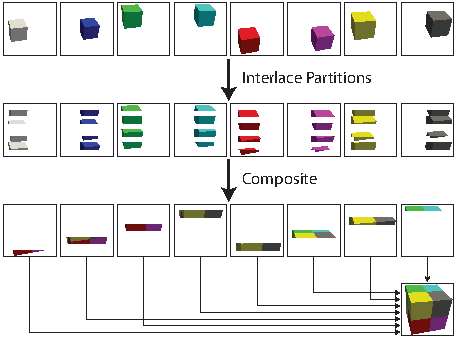
\includegraphics[width=.8\textwidth]{images/InterlaceDiagram}
  \caption{Pixel shuffling in \IceT's image interlacing.}
  \label{fig:Interlacing}
\end{figure}

\IceT's minimal-copy image interlacing is demonstrated in
Figure~\ref{fig:Interlacing}.  Rather than picking arbitrary partitions,
such as scan lines, to interlace, \IceT's interlacing uses the partitions
that the composite will create anyway.  The image with the interlaced block
is composited as normal.  Each resulting image partition is already intact,
it is only the implicit offsets that need to be adjusted.

Image interlacing is always on by default.  It can be turned off by calling
\CFunc{icetDisable} with \CEnum{ICET\_INTERLACE\_IMAGES}.  Image
interlacing is only a hint, and compositing strategies are not obligated to
follow it.  In any case, the observable behavior between interlaced and
non-interlaced images is the same except for in compositing times.  In
situations where each process renders to a small portion of an image, the
overhead for image interlacing is low but its benefits are high.  However,
in cases where every process renders geometry over the entire view
(indicative of a poor distribution of geometry), then the overhead for
image interlacing becomes higher but the benefit becomes lower.

\index{image!interlace|)}

\section{Data Replication}
\label{sec:Customizing_Compositing:Data_Replication}
\index{data~replication|(}

The primary advantage of \IceT's parallel rendering algorithms, and
sort-last rendering algorithms in general, is that they are very scalable
with respect to the size of the input geometry.  That is, there is no
overhead to adding more geometry other than the time it takes hardware to
render and there is only a logarithmic overhead for adding processors to
the job.

The down side of a sort-last approach is that the image compositing
overhead must be incurred regardless of how little geometry is being
rendered.  This overhead limits the maximum frame rate that can be achieved
by the parallel rendering.  Consequently, the parallel rendering can
potentially be slower than the serial rendering if the amount of geometry
being rendered is small.

One possible way to get higher frame rates with smaller geometries would be
to switch to a different parallel rendering mode, but doing so is
unnecessarily complicated.  Another possibility is to collect the data on
a single process and circumvent the \IceT library entirely.  This approach
is fine when using single tile mode where the image is displayed at a
single location, but is not at all straightforward when displaying to a
tiled display.

\IceT provides a better solution than either of the previous two
approaches.  If the image compositing work is dominating the rendering
time, you can set up a \keyterm{data replication group}.  To set up a data
replication group, you partition the geometry using fewer partitions than
processes, and then you share each partition with multiple processes.  The
processes that share a data partition are a replication group.  \IceT will
divide the compositing work for each replication group amongst the
processes in the group.  In essence, you are adding geometry rendering work
to remove image compositing work.

One of the most common uses for data replication groups is to simply
replicate the same geometry on all processes.  This is helpful, for
example, if your application supports lower levels of detail for
interaction.  The lower level of detail can be replicated on all
processes.  However, you could also conceivably arrange for any amount of
replication between all replicated and none replicated for a consistently
appropriate overhead as the amount of data grows.

To set up data replication groups, it is your responsibility to partition
and replicate geometry.  (\IceT knows nothing about geometry.)  You then
report what the data replication groups are with the
\CFunc{icetDataReplicationGroup} function.

\begin{Table}{3}
  \textC{void }\CFunc{icetDataReplicationGroup}\textC{(}&\textC{IceTInt}&\CArg{size}\textC{,} \\
  &\textC{const IceTInt *}&\CArg{processes}\quad\textC{);}
\end{Table}

\CFunc{icetDataReplicationGroup} simply takes an array defining the
replication group that the local process belongs to.  It is important to
ensure that all processes belonging to a group provide the same array to
\CFunc{icetDataReplicationGroup}.  As a convenience, \IceT also provides
the \CFunc{icetDataReplicationGroupColor} function that allows you to
define the data replication groups by assigning an identifier (i.e. color)
to each partition and having each process report the partition color in
which it belongs.
\begin{Table}{3}
  \textC{void }\CFunc{icetDataReplicationGroupColor}\textC{(}&\textC{IceTInt}&\CArg{color}\quad\textC{);}
\end{Table}

As an example, let us say that processes 0--3 share the same geometry, 4--7
share the same geometry, 8--11 share the same geometry, and so on.  These
replication groups could be reported with the following call (where
\textC{rank} is the local process id as stored in the \CEnum{ICET\_RANK}
state variable).
\begin{code}
icetDataReplicationGroupColor(rank/4);
\end{code}

The data replication group is stored in the
\CEnum{ICET\_DATA\_REPLICATION\_GROUP} state variable (retrievable with
\CFunc{icetGet}).  The length of the group array is stored in
\CEnum{ICET\_DATA\_REPLICATION\_GROUP\_SIZE}.  The data replication group
array is available regardless of whether you used
\CFunc{icetDataReplicationGroup} or \CFunc{icetDataReplicationGroupColor}
to define the group.  The default value is an array with one value: the
local process.

\index{data~replication|)}

\section{Drawing Callback Order}
\label{sec:Customizing_Compositing:Drawing_Callback_Order}
\index{drawing~callback|(}

The most important reason \IceT relies on a drawing callback, described in
Chapter~\ref{chap:Basic_Usage} starting on
page~\pageref{sec:Basic_Usage:Drawing_Callback}, is to allow \IceT's
compositing algorithms to minimize the number of times a render must occur
(ideally less than once per tile) and the number of pixels produced.  Thus,
\IceT will often avoid invoking the drawing callback.

Because if this, it is difficult to predict how often, if at all, the
drawing callback will be invoked on each process.  It is also difficult to
predict the order in which tiles are drawn or if the drawings will even be
aligned with the tiles.

Under most circumstances, each process can independently draw their portion
of the data, which is one of the advantages of sort-last rendering.
However, this could be problematic for some more advanced rendering
techniques that will require communication among processes.  One such
example could be a ray tracer that must communicate to find global effects
like shadows.  Another example could be a dynamically built texture like a
surface line integral convolution (or simply surface
LIC)\index{surface~LIC}.

This communication can be very difficult to implement in a draw function
that is only called on a subset of processes.  Thus some applications might
wish to force \IceT to synchronize the drawing callbacks for each tile.
This can be done by using the sequential
strategy\index{strategy!sequential}, turning off floating
viewports\index{floating~viewport}, and turning on the option to render
empty images (even though the result will be ignored).  The following code
performs all these actions.

\index{icetStrategy}
\index{ICET\_STRATEGY\_SEQUENTIAL}
\index{ICET\_FLOATING\_VIEWPORT}
\index{ICET\_RENDER\_EMPTY\_IMAGES}
\begin{code}
icetStrategy(ICET_STRATEGY_SEQUENTIAL);
icetDisable(ICET_FLOATING_VIEWPORT);
icetEnable(ICET_RENDER_EMPTY_IMAGES);
\end{code}

Keep in mind that all of these options are turning off many of the
optimizations \IceT uses during compositing.  If rendering a single tile,
the effect is likely negligible, but the cost rises steeply as more tiles
are added to the display.

\index{drawing~callback|)}

\section{Compositing Network Hints}
\label{sec:Customizing_Compositing:Compositing_Network_Hints}
\index{compositing!network|(}

By its nature, image compositing requires a significant amount of
communication amongst processes in a parallel computer.  Each compositing
algorithm contained in \IceT follows a particular pattern of communication,
referred to as its \keyterm{compositing network}.  These algorithms and
their compositing networks are described in Chapter~\ref{chap:Strategies}.

Most compositing networks are fixed although a few have some possible
variability.  Any variations in the compositing networks are automatically
chosen, but it is possible to provide hints.  Because the relative
efficiency of different compositing networks is effected more by the
underlying hardware than in the application and data running it, these hints
are specified by either build options or by environment variables.

Build options are specified as \index{CMake}CMake variables.  These CMake
variables are set using the CMake program at the beginning of the build as
described in Chapter~\ref{chap:Tutorial}.  These variables are listed as
``advanced,'' so you will need to turn on advanced variables in the CMake
to see them.

For each one of these CMake build variables, \IceT also recognizes a
corresponding environment variable with the same name at run time.  If the
environment variable is defined, it will be used in place of the option set
at run time.  The environment variables are read when the \IceT context is
first created, so subsequent changes to the environment variables will have
no effect.

The following CMake and environment variable hints are available.

\begin{Description}[xxxxxxxx]
\item[\CEnum{ICET\_MAGIC\_K}] The radix-k single image strategy described
  in Chapter~\ref{chap:Strategies} starting on
  page~\pageref{sec:Strategies:Radix-k} operates by communicating within
  groups of processes of size $k$.  \IceT's implementation of radix-k
  automatically determines $k$, but does so by selecting values that are as
  close as possible to a \index{magic~k}\keyterm{magic k} value.  This
  magic k value is set with the \CEnum{ICET\_MAGIC\_K} CMake build variable
  or environment variable.
\item[\CEnum{ICET\_MAX\_IMAGE\_SPLIT}] The parallel image compositing
  algorithms in \IceT maintain load balancing by dividing images amongst
  processes to allow the processes to concurrently composite pixels in
  independent partitions of the image.  Typically, \IceT subsequently
  collects the images to the display nodes.  This collection can be one of
  the longest operations during the compositing, particularly when there
  are many processes.  It is possible to speed up the collection at the
  expense of the compositing by limiting the maximum number of times an
  image may be split.  This limit is set with the
  \CEnum{ICET\_MAX\_IMAGE\_SPLIT} CMake build variable or environment
  variable.  Be advised that this option is only a suggestion to
  compositing.  It is still possible for images to be split beyond this
  limit.  \IceT will still behave correctly either way.
\end{Description}

These values may be queried (but not set) at runtime using \CFunc{icetGet}
with a state variable identifier of the same name.

\index{compositing!network|)}

\section{Image Partition Collection}
\label{sec:Customizing_Compositing:Image_Collection}
\index{collection|(}
\index{image!collection|(}
\index{partitioning!image|(}
\index{image!partitioning|(}

Many parallel compositing algorithms, including several in \IceT, function
by partitioning images and distributing the pieces.  These algorithms,
described in more detail in Chapter~\ref{chap:Strategies}, eventually have
a composited image partitioned and distributed among most or all of the
processes involved in the operation.

For most practical purposes, such as displaying the images, the image
partitions must be collected, and by default \IceT collects each image to
its associated display process.  However, there exist some use cases where
this collection may not be necessary.  For example, if the images are only
to be written to a parallel file system, then it may be as efficient or
more efficient to collectively write partitions from multiple processes.

The collection of image data to the display process may take a significant
portion of the overall compositing time, but it is usually necessary.  When
it is not necessary, it can be disabled by calling \CFunc{icetDisable} with
\CEnum{ICET\_COLLECT\_IMAGES}.  When this option is turned off, the
strategy has the option of leaving images partitioned among processes.
Each process containing part of a tile's image will return the entire
buffer from \CFunc{icetDrawFrame}, \CFunc{icetCompositeImage}, or
\CFunc{icetGLDrawFrame} in an \CType{IceTImage} object.  However, only
certain pixels will be valid.  The state variables
\CEnum{ICET\_VALID\_PIXELS\_TILE}, \CEnum{ICET\_VALID\_PIXELS\_OFFSET}, and
\CEnum{ICET\_VALID\_PIXELS\_NUM} give which tile the pixels belong to and
what range of pixels are valid.

The \CEnum{ICET\_VALID\_PIXELS\_TILE} state variable gives the tile for
which the last image returned from \CFunc{icetDrawFrame},
\CFunc{icetCompositeImage}, or \CFunc{icetGLDrawFrame} contains pixels.
Each process has its own value.  If the last call to \CFunc{icetDrawFrame},
\CFunc{icetCompositeImage}, or \CFunc{icetGLDrawFrame} did not return
pixels for the local process, then this state variable is set to $-1$.

The \CEnum{ICET\_VALID\_PIXELS\_OFFSET} and
\CEnum{ICET\_VALID\_PIXELS\_NUM} give the range of valid pixels for the
last image returned from \CFunc{icetDrawFrame}, \CFunc{icetCompositeImage},
or \CFunc{icetGLDrawFrame}.  Given the arrays of pixels returned with the
\CFunc{icetImageGetColor} and \CFunc{icetImageGetDepth} functions, the
valid pixels start at the pixel indexed by
\CEnum{ICET\_VALID\_PIXELS\_OFFSET} and continue for
\CEnum{ICET\_VALID\_PIXELS\_NUM}.  The tile to which these pixels belong
are captured in the \CEnum{ICET\_VALID\_PIXELS\_TILE} state variable.  If
the last call to \CFunc{icetDrawFrame}, \CFunc{icetCompositeImage}, or
\CFunc{icetGLDrawFrame} did not return pixels for the local process,
\CEnum{ICET\_VALID\_PIXELS\_NUM} is set to $0$.

The \CEnum{ICET\_VALID\_PIXELS\_TILE}, \CEnum{ICET\_VALID\_PIXELS\_OFFSET},
and \CEnum{ICET\_VALID\_PIXELS\_NUM} are only really useful when
\CEnum{ICET\_COLLECT\_IMAGES} is disabled.  When
\CEnum{ICET\_COLLECT\_IMAGES} is enabled, it is always the case that each
display process has the entire image (\CEnum{ICET\_VALID\_PIXELS\_TILE} set
to the tile, \CEnum{ICET\_VALID\_PIXELS\_OFFSET} set to $0$ and
\CEnum{ICET\_VALID\_PIXELS\_NUM} set to the total image size), and it is
always the case that each process not displaying a tile has no image
(\CEnum{ICET\_VALID\_PIXELS\_TILE} set to $-1$ and
\CEnum{ICET\_VALID\_PIXELS\_NUM} set to $0$).

\index{image!partitioning|)}
\index{partitioning!image|)}
\index{image!collection|)}
\index{collection|)}

\section{Timing (and Other Metrics)}
\label{sec:Customizing_Compositing:Timing}
\index{timing|(}

Whenever \CFunc{icetDrawFrame}, \CFunc{icetCompositeImage}, or
\CFunc{icetGLDrawFrame} is called, \IceT measures the amount of time spent
in the various tasks required for parallel rendering.  These timings are
stored in the \IceT state and can be retrieved with \CFunc{icetGet}.  The
state variables containing these timing metrics (in seconds) are as
follows.

\begin{Description}[xxxxxxxx]
\item[\CEnum{ICET\_RENDER\_TIME}] The total time spent in the drawing
  callback during the last call to \CFunc{icetDrawFrame} or
  \CFunc{icetGLDrawFrame}. Always set to 0.0 after a call to
    \CFunc{icetCompositeImage}.
\item[\CEnum{ICET\_BUFFER\_READ\_TIME}] The total time spent copying buffer
  data and reading from \OpenGL buffers during the last call to
  \CFunc{icetDrawFrame}, \CFunc{icetCompositeImage}, or
  \CFunc{icetGLDrawFrame}.
\item[\CEnum{ICET\_BUFFER\_WRITE\_TIME}] The total time spent writing to
  OpenGL buffers during the last call to \CFunc{icetGLDrawFrame}.  Always
  set to 0.0 after a call to \CFunc{icetDrawFrame} or
  \CFunc{icetCompositeImage}.
\item[\CEnum{ICET\_COMPRESS\_TIME}] The total time spent in compressing
  image data using active pixel encoding during the last call to
  \CFunc{icetDrawFrame}, \CFunc{icetCompositeImage}, or
  \CFunc{icetGLDrawFrame}.
\item[\CEnum{ICET\_BLEND\_TIME}]/\CEnum{ICET\_COMPARE\_TIME} The total time
  spent in performing Z comparisons or color blending of images during the
  last call to \CFunc{icetDrawFrame}, \CFunc{icetCompositeImage}, or
  \CFunc{icetGLDrawFrame}.  These two variables always return the same
  value.
\item[\CEnum{ICET\_COLLECT\_TIME}] The total time spent in collecting image
  fragments to display processes during the last call to
  \CFunc{icetDrawFrame}, \CFunc{icetCompositeImage}, or
  \CFunc{icetGLDrawFrame}.
\item[\CEnum{ICET\_TOTAL\_DRAW\_TIME}] The total time spent in the last
  call to \CFunc{icetDrawFrame}, \CFunc{icetCompositeImage}, or
  \CFunc{icetGLDrawFrame}.  This includes all the time to render, read
  back, compress, and composite images.
\item[\CEnum{ICET\_COMPOSITE\_TIME}] The total time spent in compositing
  during the last call to \CFunc{icetDrawFrame},
  \CFunc{icetCompositeImage}, or \CFunc{icetGLDrawFrame}.  Equal to
  $\CEnum{ICET\_TOTAL\_DRAW\_TIME} - \CEnum{ICET\_RENDER\_TIME} -
  \CEnum{ICET\_BUFFER\_READ\_TIME} - \CEnum{ICET\_BUFFER\_WRITE\_TIME}$.
\end{Description}

In addition to timing how long rendering and compositing takes, \IceT also
keeps track of how much data is transmitted during compositing.  The state
variable \CEnum{ICET\_BYTES\_SENT} stores the total number of bytes sent by
the calling process for transferring image data during the last call to
\CFunc{icetDrawFrame}, \CFunc{icetCompositeImage}, or
\CFunc{icetGLDrawFrame}.  Obviously, each process could have a different
value for \CEnum{ICET\_BYTES\_SENT}.

\IceT also keeps track of the number of times \CFunc{icetDrawFrame},
\CFunc{icetCompositeImage}, or \CFunc{icetGLDrawFrame} has been called.
This number is stored in \CEnum{ICET\_FRAME\_COUNT}.

\index{timing|)}


% -*- Index -*-


\chapter{Strategies}
\label{chap:Strategies}

\index{strategy|(}

\IceT contains several parallel image compositing algorithms.  The type of
compositing algorithm to use is selected by choosing a
\index{strategy}\keyterm{strategy}.  This chapter describes the underlying
algorithm of each strategy.  This user's guide will give qualitative
comparisons between the strategies, but for a more quantitative analysis,
see the following paper.

\begin{quote}
  Kenneth Moreland, Brian Wylie, and Constantine Pavlakos.  ``Sort-last
  parallel rendering for viewing extremely large data sets on tile
  displays,'' In \emph{Proceedings of IEEE Symposium on Parallel and
    Large-Data Visualization and Graphics}, October 2001, pp. 85--154.
\end{quote}

A strategy is specified using the \CFunc{icetStrategy} function.

\begin{Table}{3}
  \textC{void }\CFunc{icetStrategy}\textC{(}&\CType{IceTStrategy}&\CArg{strategy}\quad\textC{);}
\end{Table}

The \CArg{strategy} is set to one of the identifiers for the strategies
documented in the following sections of this chapter.  A string documenting
the current strategy can be retrieved with the \CFunc{icetGetStrategyName}
function.

To describe the \IceT compositing algorithms, we will use the example
parallel rendering problem shown in Figure~\ref{fig:ExampleInputs} where 6
processes are each rendering their own piece of a shuttle model to a two
tile display.

\begin{figure}
  \centering
  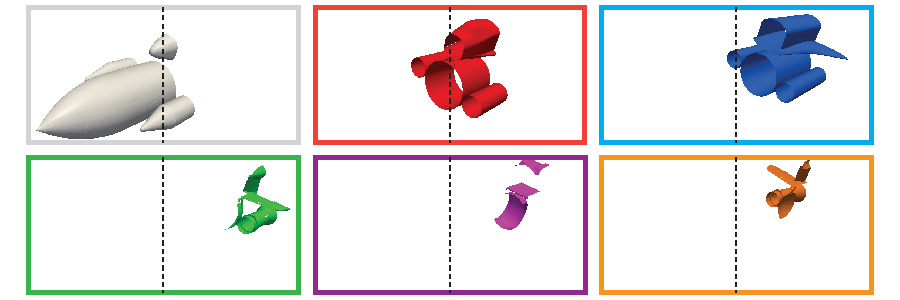
\includegraphics{images/AllInput}
  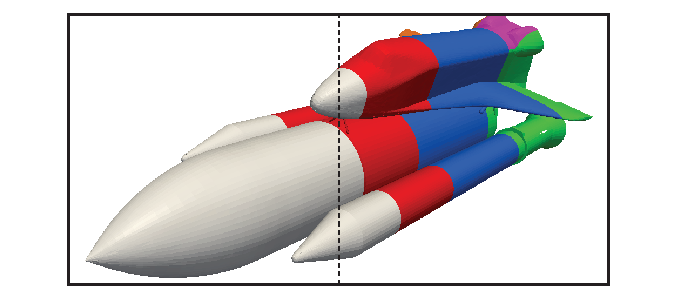
\includegraphics{images/CompositedInput}
  \caption[Example compositing problem.]{An example of six processes
    rendering to two tiles (top) and their composited image (bottom).}
  \label{fig:ExampleInputs}
\end{figure}

In this example, processes are denoted, in no particular order, by the
colors gray, red, blue, green, purple, and orange.  The colors of the
geometry correspond to the process that generated each piece.  Image
boarder colors denote the process that generates and holds that image.
(Apologies to those having troubles resolving the colors due to poor
display or vision deficiencies.  It should not be hard to follow the
descriptions either way.)

\section{Single Image Compositing}

\index{single~image~composite|(}
\index{compositing!single~image|(}

Before discussing the multi-tile image compositing algorithms implemented
by \IceT, we visit the standard single image compositing algorithms.  You
cannot directly select a single image compositing algorithm as a strategy
(most of the multi-tile algorithms work well in ``single-tile'' mode), but
these compositing algorithms are used as ``subroutines'' in some of the
multi-tile algorithms.  A reference to a
\index{single~image~composite~network}\keyterm{single image composite
  network} in the subsequent compositing algorithm descriptions refers to
the algorithms described here.

\subsection{Tree Compositing}

\index{compositing!tree|(}
\index{tree~composite|(}
\index{binary~tree~composite|(}

\IceT internally has two single image composite implementations.  The first
of which is the \keyterm{tree composite} algorithm (sometimes also called
binary tree composite due to its pair-wise grouping).  The basic network
for tree composite is shown in Figure~\ref{fig:BinaryTree}.

\begin{figure}
  \centering
  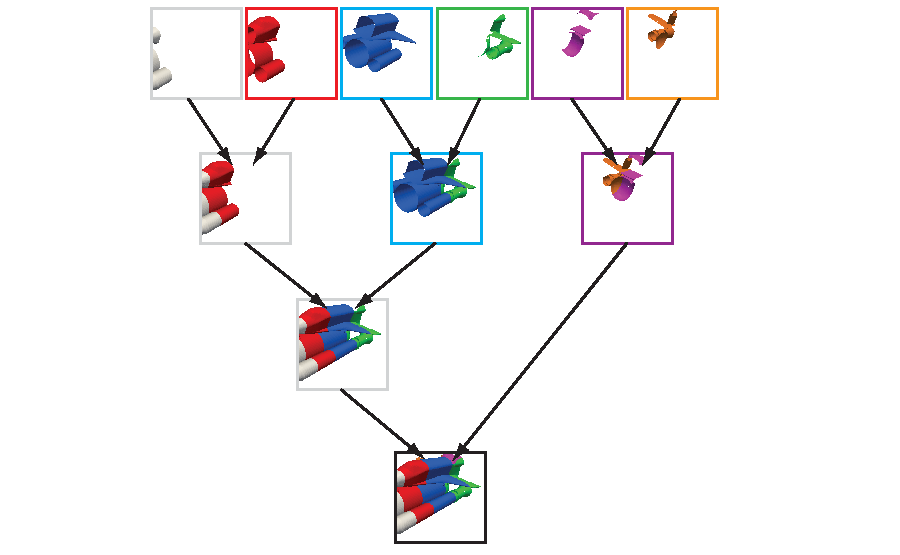
\includegraphics{images/BinaryTree}
  \caption[Tree composite network.]{Tree composite network.  Arrows
    represent the passing of data from one stage to the next.  Processes
    receiving multiple images composite them together.}
  \label{fig:BinaryTree}
\end{figure}

The tree compositing algorithm is organized in stages.  At each stage the
processes pair up.  One of the processes sends its data to its pair and
then drops out of the computation.  The receiving process combines the two
images (using the \index{compositing~operation}compositing operation
described in
Chapter~\ref{sec:Customizing_Compositing:Compositing_Operation}) and
continues to the next stage.  Processing continues until there is only one
image (and one process) remaining.

As just defined, the tree composite algorithm only handles process counts
that are a power of two (that is, the number of processes is equal to $2^i$
for some integer $i$).  \IceT handles non-powers of two gracefully.  At any
stage where the number of processes is not even and one of the processes
cannot be paired, that leftover process does nothing for that stage but
then continues to participate in the next stage.  An example of this can be
seen in the second stage of Figure~\ref{fig:BinaryTree}.

The advantages of tree composite are its regular and efficient data
transfers.  The limiting factor of tree compositing is that at each stage
of the algorithm half of the processes drop out of the computation.  Thus,
for more than a few processes tree compositing provides poor process
utilization.

\index{binary~tree~composite|)}
\index{tree~composite|)}
\index{compositing!tree|)}

\subsection{Binary-Swap Compositing}

\index{compositing!binary~swap|(}
\index{binary~swap~composite|(}

The second single image compositing algorithm used internally by \IceT is
the \keyterm{binary swap} algorithm.  The basic network for binary-swap
composite is shown in Figure~\ref{fig:BinarySwap}

\begin{figure}
  \centering
  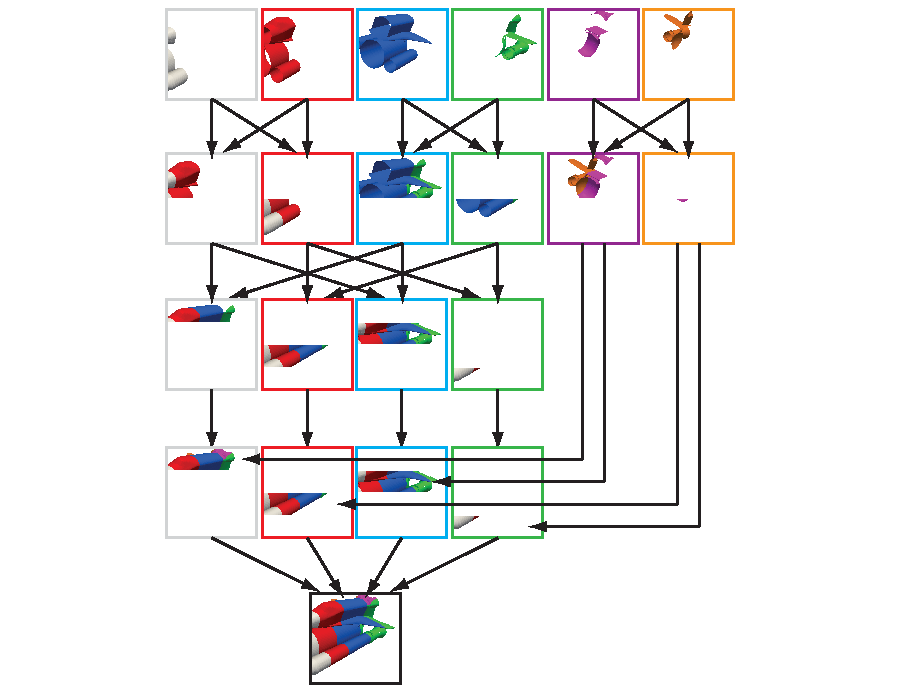
\includegraphics{images/BinarySwap}
  \caption[Binary-swap composite network.]{Binary-swap composite network.
    Arrows represent the passing of data from one stage to the next.
    Processes receiving multiple images composite or stitch them together.
    At most stages each process divides its image data and distributes it.
    The distribution of image data can be inferred from the target images.}
  \label{fig:BinarySwap}
\end{figure}

Like tree compositing, binary swap is organized in stages, and at each
stage the processes pair up.  However, rather than have one process send
all the data to the other, the image space is divided in two and the
processes swap image data so that each process has all the data for part of
the image.  At the next stage, the processes pair up again, but with
different partners that have the same partition of the image.  Processing
continues until each of the $N$ processes have an image $1/N$ the size of
the original image.  At this point, all the processes send their sub-image
to the display processes where the images are stitched together.

As just defined, the binary-swap composite algorithm only handles processes
that are a power of two (that is, the number of processes is equal to $2^i$
for some integer $i$).  Some binary-swap implementations handle non-powers
of two by reducing the problem to the next largest power of two and
dropping the leftover processes, but \IceT handles non-powers of two more
gracefully than that.  Instead, \IceT first finds the largest group of
processes that is a power of two, makes a partition out of them, then finds
the next largest group of processes that remain that is a power of two,
makes a partition out of them, and so on.  Each partition runs binary-swap
independently up to the point where each process has its own piece of data.
At this point, the smaller partitions send their image data to processes of
the larger partitions, dividing up images where necessary.  The largest
partition then finishes the compositing in the normal way by collecting all
of the pieces.

An example of compositing with a non-power of two is given in
Figure~\ref{fig:BinarySwap}.  The six processes are partitioned first into
a group of 4 and then into a group of 2.  After swapping, the processes in
the smaller group send images to the larger group.  In this case, the purple
process sends image data to the gray and blue processes, and the orange
process sends to the red and green processes.

Like tree composite, binary swap exhibits regular and efficient data
transfers.  In addition, binary swap involves the use of all the processes
throughout most of the compositing.  Consequently, binary swap exhibits
very good process utilization and scaling with respect to the number of
processes on which it is run.

The most inefficient part of binary swap is the collection of image
fragments at the end, which is an extra step that tree composite does not
need to take.  Through some empirical studies, we found that the binary
tree algorithm was more efficient than binary swap on less then 8 processes and
less efficient on more than 8 processes.  Consequently, \IceT automatically
switches between the two algorithms based on the amount of processes
involved in the compositing.

\index{binary~swap~composite|)}
\index{compositing!binary~swap|)}

\subsection{Ordered Compositing}

\index{compositing!ordered|(}

In some applications, the order in which images are composited together
makes a difference (see the Volume Rendering section in
Chapter~\ref{sec:Customizing_Compositing:Volume_Rendering}).  The details
on how ordered compositing is achieved is not given here, but the basic
idea for both compositing algorithms is that they first swizzle the
processes so that their order matches the order in which the images need to
be composited together.  When compositing images together, they make sure
to maintain over/under constancy based on the swizzled ranks from the
originating processes.  The networks are also managed such that no two
images are composited that are not directly ``next'' to each other (that
is, there is no image that needs to be inserted between them).

\index{compositing!ordered|)}

\index{compositing!single~image|)}
\index{single~image~composite|)}

\section{Reduce Strategy}
\label{sec:Strategies:Reduce}

\index{strategy!reduce|(}
\index{reduce~strategy|see{strategy, reduce}}
\index{reduce~to~single~tile|see{strategy, reduce}}

An effective strategy implemented in \IceT is the \keyterm{reduce to single
  tile strategy} (or simply the reduce strategy).  In this strategy, the
multi-tile composite problem is efficiently reduced to a set of single
image compositing problems, which are well studied and discussed in the
previous section.  The reduce strategy is selected by calling
\CFunc{icetStrategy} with the \CEnum{ICET\_STRATEGY\_REDUCE} argument.

\begin{figure}
  \centering
  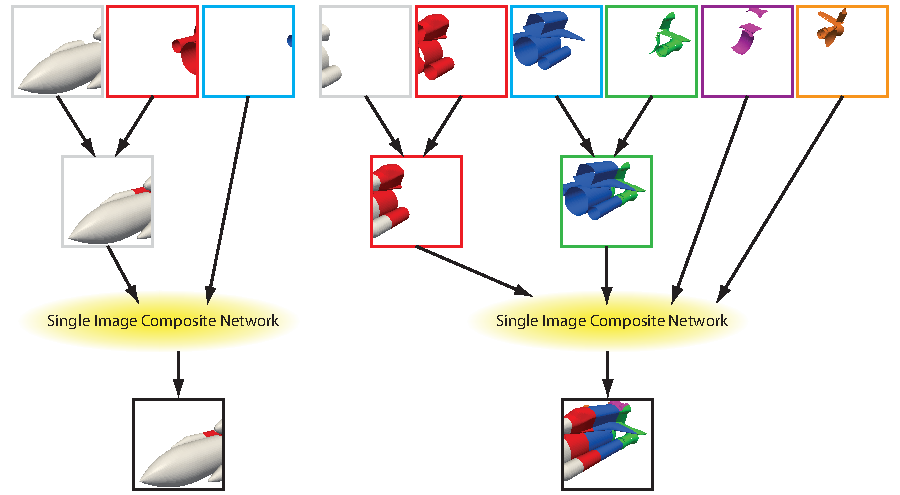
\includegraphics{images/ReduceComposite}
  \caption[Reduce strategy composite network.]{Composite network for reduce
    strategy.  Arrows represent the passing of data from one stage to the
    next.  Processes receiving multiple images composite them together.
    The single image composite network is described in a preceding
    section.}
  \label{fig:ReduceComposite}
\end{figure}

The reduce strategy is performed in two phases.  In the first phase,
processes are partitioned into groups, each of which is responsible for
compositing the image of one of the tiles.  The number of processes
assigned to each tile is proportional to the number of non-empty images
rendered for the corresponding tile.  In the example shown in
Figure~\ref{fig:ReduceComposite} there are a total of 9 non-empty images.
The left tile has 3 of the 9, that is $\frac{1}{3}$, of the images and thus
is assigned $\frac{1}{3} \times 6 = 2$ processes.  Likewise, the right
image is assigned $\frac{2}{3} \times 6 = 4$ processes.

When assigned processes to tiles, display processes and processes rendering
images to the tile are given preference.  In the example of
Figure~\ref{fig:ReduceComposite}, the gray and blue processes are assigned
to the left tile.  The remainder are assigned to the right tile.  Any image
generated by a process that does not belong to the destination tile is
transferred to a process assigned to the tile.  In the example, the three
processes that render two images, gray, red, and blue, each pass one of
their images to a process in the opposing process group.  All of these
transfers have unique senders and receivers and thus can happen
simultaneously.

In the second phase of the reduce strategy, each group of processes
independently composites its images together using one of the single image
compositing algorithms described in the preceding section.

The reduce strategy supports ordered compositing.  It does this by ensuring
in the first phase that processes receive only images that are ``near'' the
image they hold, that is, there is no other image in between the two images
in the visibility ordering.  The single image compositing algorithms of the
second phase each support their own ordered compositing.

\index{strategy!reduce|)}

\section{Split Strategy}
\label{sec:Strategies:Split}

\index{strategy!split|(}
\index{split~strategy|see{strategy, split}}
\index{tile~split~and~delegate|see{strategy, split}}

The \keyterm{tile split and delegate strategy} (or simply the split
strategy) is a simple algorithm that splits up tiles, assigns each piece to
a tile, and then sends image fragments directly to the tiles for
compositing.  The split strategy makes efficient use of processing
resources, but exhibits haphazard message passing which can cause issues on
some high speed interconnects.  The split strategy is selected by calling
\CFunc{icetStrategy} with the \CEnum{ICET\_STRATEGY\_SPLIT} argument.

\begin{figure}
  \centering
  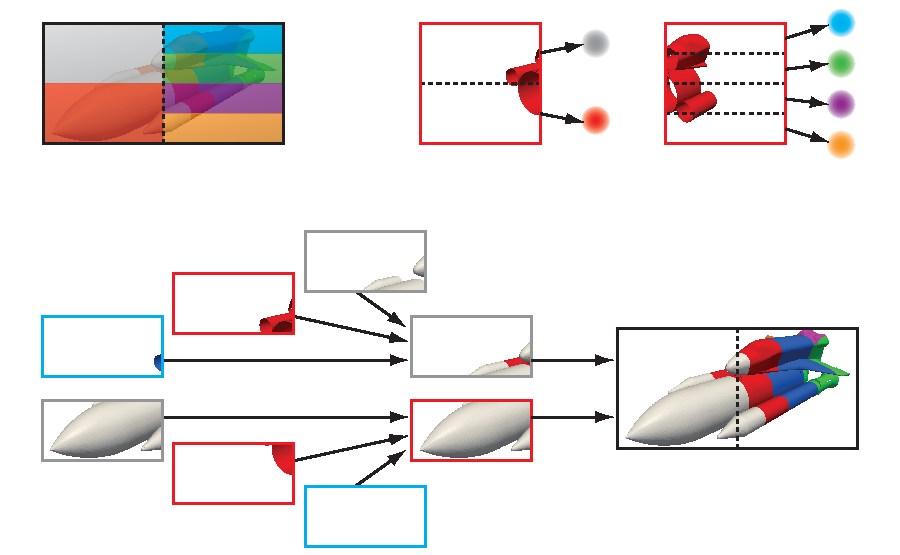
\includegraphics{images/TileSplit}
  \caption[Split strategy composite network.]{Compositing for split
    strategy.  First tiles are split and assigned to processes (upper
    left).  Then each process simultaneously sends its images to the
    responsible process (upper right) and receives all sub-images for its
    piece (bottom).  The composited pieces are then collected and stitched
    together.}
  \label{fig:TileSplit}
\end{figure}

The split strategy first assigns processes to tiles similar to how they are
assigned in the reduce strategy described previously.  That is, the number
of processes per tile is proportional to the number of non-empty images
generated for it.  Each tile is then split up evenly amongst all processes
assigned to it.  In the example in Figure~\ref{fig:TileSplit}, the upper
left image shows that the left image is split between 2 processes and the
right image is split amongst 4 processes.

On being assigned a section of tile, each process prepares to receive data
from all the sending processes using asynchronous receives.  Each process
then renders its images, splits them up, and sends the sub-images to the
corresponding process.  When a process is ready and as it receives data,
the incoming images are composited together.  Once all of the incoming
images are composited, the complete sub-image is sent to the display process
to be stitched together.

The split strategy does not support ordered compositing.  Using the split
strategy in color blending mode will fail.

\index{strategy!split|)}

\section{Virtual Trees Strategy}
\label{sec:Strategies:Vertial_Trees}

\index{strategy!virtual~trees|(}
\index{virtual~trees|see{strategy, virtual trees}}

The \keyterm{virtual trees strategy} is based on the binary tree
compositing algorithm, but performs multiple composites simultaneously to
regain some of the load balance lost in the original algorithm.  The
virtual trees strategy has nice regular communications, but still suffers
from some load imbalance, particularly when using fewer tiles and in later
stages of the algorithm.  The virtual trees strategy is selected by calling
\CFunc{icetStrategy} with the \CEnum{ICET\_STRATEGY\_VTREE} argument.

\begin{figure}
  \centering
  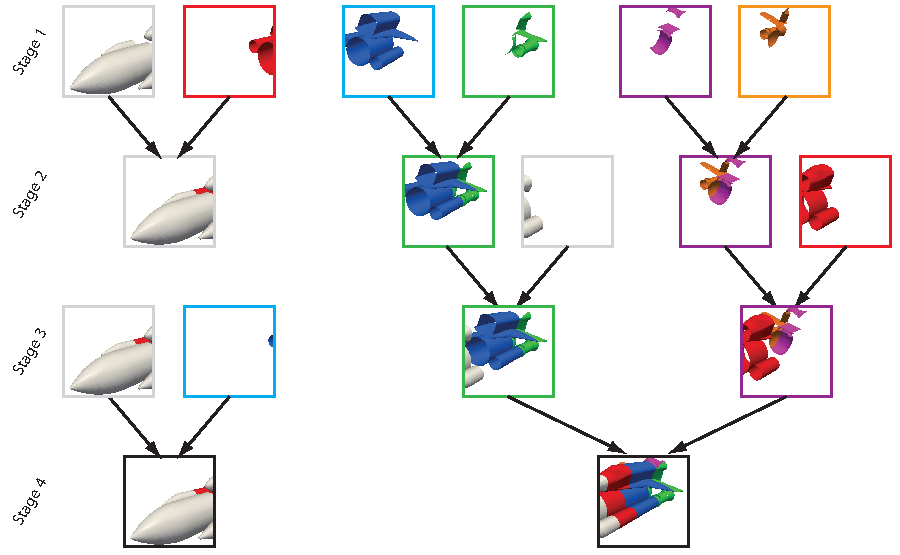
\includegraphics{images/VTrees}
  \caption[Virtual trees composite network.]{Composite network for virtual
    trees strategy.  Arrows represent the passing of data from one state to
    the next.  Processes receiving multiple images composite them
    together.}
  \label{fig:VTreesComposite}
\end{figure}

The virtual trees strategy works by creating a ``virtual'' tree for each
tile.  Contained in each tree are processes that have rendered an image for
that display tile.  The algorithm proceeds much like the binary tree
composition algorithm except that the processes float amongst the trees,
helping with the compositing as they become available.
Figure~\ref{fig:VTreesComposite} shows an example of the virtual trees
compositing.  In particular, notice that the gray process takes part in the
left tree in stage 1, then floats to take part in the right tree in stage
2, and then returns to take part in the left tree in stage 3.

When necessary, the process must keep track of multiple images belonging to
different virtual trees.  Two conserve memory, images are not rendered
until they are needed.  Also, a process can only hold two images at a time:
one that it is sending and one that it is receiving.  If a process is
holding an image for one tile, it cannot receive an image for another tile
until it sends away the image it is holding.

The virtual trees strategy does not support ordered compositing.  Using the
virtual trees strategy in color blending mode will fail.

\index{strategy!virtual~trees|)}

\section{Serial Strategy}
\label{sec:Strategies:Serial}

\index{strategy!serial|(}
\index{serial~strategy|see{strategy, serial}}

Despite its name, the \keyterm{serial strategy} does not completely
serialize the image compositing process.  Rather, it serially addresses the
tiles, but performs parallel compositing for each tile.  The serial
strategy is selected by calling \CFunc{icetStrategy} with the
\CEnum{ICET\_STRATEGY\_SERIAL} argument.

\begin{figure}
  \centering
  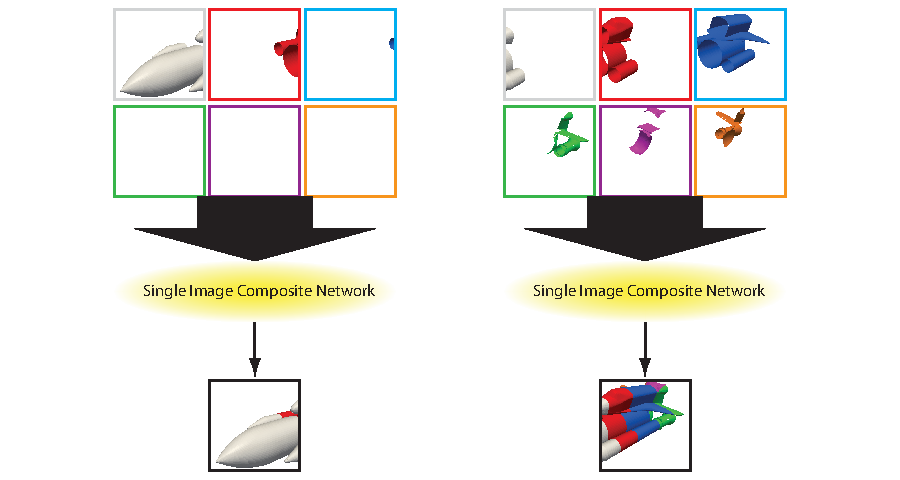
\includegraphics{images/SerialComposite}
  \caption[Serial compositing network.]{Composite network for serial
    compositing.  One at a time, each tile is composited using a parallel
    single image composite network described in a previous section.}
  \label{fig:SerialComposite}
\end{figure}

The serial strategy iterates over all of the tiles.  For each tile, it
composites all the images for that tile using one of the single image
compositing algorithms described in that preceding section.  As
demonstrated in the example in Figure~\ref{fig:SerialComposite} images from
all processes are composited for each tile regardless of whether some of
them may be empty.

Since the single image compositing algorithms support ordered
compositing, the serial strategy also supports ordered compositing.

The serial strategy is really only implemented as a baseline algorithm to
compare other algorithms.  In general, the reduce strategy does at least as
well or outperforms the serial strategy.  We have observed this even in
single tile mode, possibly because the reduce strategy can throw away empty
images.

\index{strategy!serial|)}

\section{Direct Send Strategy}
\label{sec:Strategies:DirectSend}

\index{strategy!direct~send|(}
\index{direct~send~strategy|see{strategy, direct send}}

The \keyterm{direct send strategy} is the simplest of all the strategies.
Each process simply renders its images and sends them directly to the
display process where the images get composited, as shown in
Figure~\ref{fig:DirectSend}.  The direct send strategy is selected by
calling \CFunc{icetStrategy} with the \CEnum{ICET\_STRATEGY\_DIRECT}
argument.

\begin{figure}
  \centering
  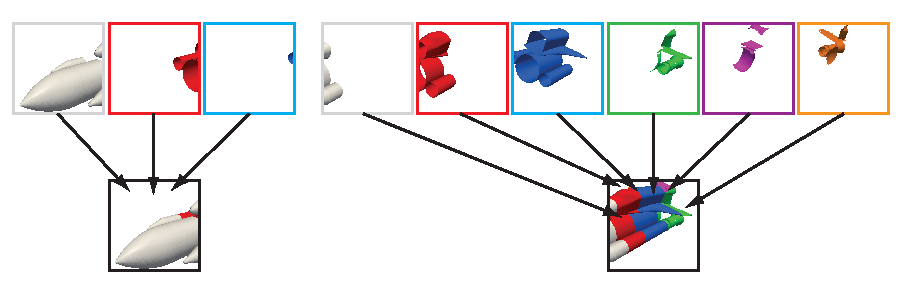
\includegraphics{images/DirectSend}
  \caption[Direct send compositing network.]{Composite network for direct
    send compositing.  Arrows represent the passing of data from one
    process to another.  Receiving process composite all incoming images
    together.}
  \label{fig:DirectSend}
\end{figure}

The direct send strategy is usually a poor performer.  It was designed as a
low watermark to compare to other compositing strategies.  The direct send
strategy does, however, support ordered compositing.

\index{strategy!direct~send|)}

\section{Implementing New Strategies}

The \IceT API was writen while its strategies were being developed.  As
such, the design yields for the relatively simplistic addition of new
strategies.  This section will provide the basic overview of how to add a
new strategy.  It is probably easiest to start by modifying your \IceT
source to insert your own strategy in the src/ice-t/strategies directory of
the \IceT source distribution.  It should be possible to create an external
library with a strategy in it, but there may be some complications with
finding include files and getting the proper exports.

A strategy in \IceT is created by simply defining an \CType{IceTStrategy}
object.  The \CType{IceTStrategy} type is generally meant to be an opaque
type so that most users to not have to be concerned with the strategy
innards.  However, the \IceT code base is currently quite stable and the
\CType{IceTStrategy} type rarely changes in any case.

The \CType{IceTStrategy} type is defined in the
\index{ice-t.h}\index{GL/ice-t.h}\textC{GL/ice-t.h} header file.
\begin{code}
typedef GLuint *IceTImage;
typedef struct _IceTStrategy {
    const char *name;
    GLboolean supports_ordering;
    IceTImage (*compose)(void);
} IceTStrategy;
\end{code}
The \textC{name} field in the \CType{IceTStrategy} type is a short string
identifying the strategy.  (It is the string returned by
\CFunc{icetGetStrategyName} when the strategy is active.)  The
\textC{supports\_ordering} field is a boolean value indicating whether the
strategy supports ordered compositing.  Finally, and most importantly, the
\textC{compose} field is a function that is called during an invocation of
\CFunc{icetDrawFrame} to perform the rendering and compositing.  It takes
no arguments (the composition should rely on the current \IceT state), and
returns a composited image.  The proper format for the \CType{IceTImage}
returned is discussed later.

All it takes to make \IceT use a new strategy is to define and fill an
object of type \CType{IceTStrategy} and pass it to the \CFunc{icetStrategy}
function.  Typically this is done as a static object somewhere within your
library source.  For example, the declaration for the direct send strategy
looks like this.

\begin{code}
static IceTImage directCompose(void);

IceTStrategy ICET_STRATEGY_DIRECT = { "Direct", ICET_TRUE, directCompose };
\end{code}

The object is also exposed in the
\index{ice-t.h}\index{GL/ice-t.h}\textC{GL/ice-t.h} header file in a way
that does not require linking directly to the strategy function.
\begin{code}
ICET_STRATEGY_EXPORT extern IceTStrategy ICET_STRATEGY_DIRECT;
\end{code}

The \CEnum{ICET\_STRATEGY\_DIRECT} name is intentionally formed to look
like a C macro for an identifier, and it is entended to be used by the end
user as such.  (\CEnum{ICET\_STRATEGY\_EXPORT} is a real C macro that
performs library export magic.)  Your strategy should define a
\CType{IceTStrategy} in a similar manner.  The remainder of this section
describes how to implement the compose function.

\subsection{Internal State Variables for Compositing}

As stated previously, a strategy's compose function does not take any
arguments.  Instead, it gets all relevant information from the \IceT state.
Many of the relevant state variables are described in the documentation for
the \CFunc{icetGet} functions (as well as elsewhere throughout this
document).  There are also several ``hidden'' state variables for internal
use.  The ones specifically useful for within a composite function are
listed here (along with the variable type, number of entries, and a
description).  Note that these state variables generally should be read
from, not written to.

\begin{Description}[xxxxxxxx]
\item[\CEnum{ICET\_ALL\_CONTAINED\_TILES\_MASKS}] (boolean,
  \CEnum{ICET\_NUM\_TILES} $\times$ \CEnum{ICET\_NUM\_PROCESSES}) Contains
  an appended list of \CEnum{ICET\_CONTAINED\_TILES\_MASK} variables for
  all processes.  Given process $p$ and tile $t$, the entry at
  $p+\CEnum{ICET\_NUM\_TILES} \times t$ contains the flag describing
  whether process $p$ renders a non-blank image for tile $t$.  This
  variable is the same on all processes.
\item[\CEnum{ICET\_CONTAINED\_TILES\_LIST}] (integer,
  \CEnum{ICET\_NUM\_CONTAINED\_TILES}) All the tiles into which the local
  geometry projects.  In other words, this is the list of tiles which will
  not be empty after local rendering.  The local processor should generate
  images for these tiles and participate in the composition of them.
\item[\CEnum{ICET\_CONTAINED\_TILES\_MASK}] (boolean,
  \CEnum{ICET\_NUM\_TILES}) This is a list of boolean flags, one per tile.
  The flag is 1 if the local geometry projects onto the tile (that is, the
  local render will not be empty for that tile) and 0 otherwise.  This
  gives the same information as \CEnum{ICET\_CONTAINED\_TILES\_LIST}, but
  in a different way that can be more convenient in some circumstances.
\item[\CEnum{ICET\_CONTAINED\_VIEWPORT}] (integer, 4) Describes the region
  of the viewport that the geometry being rendered locally projects onto.
  The bounds of the data (given by \CFunc{icetBoundingBox} or
  \CFunc{icetBoundingVertices}) onto the tile display and determines the
  region of the tile display the data covers.  The values in the four-tuple
  correspond to x, y, width, and height, respectively, of the projection in
  global pixel coordinates.  This variable in conjunction with the
  \CEnum{ICET\_NEAR\_DEPTH} and \CEnum{ICET\_FAR\_DEPTH} give the full 3D
  projection of the local data in window space.
\item[\CEnum{ICET\_FAR\_DEPTH}] (double, 1) The maximum depth value of the
  local geometry after projection.  See \CEnum{ICET\_CONTAINED\_VIEWPORTS}
  for more details.
\item[\CEnum{ICET\_IS\_DRAWING\_FRAME}] (boolean, 1) Set to true while in a
  call to \CFunc{icetDrawFrame} and set to false otherwise.  This should
  always be set to true while the compose function is being executed.
\item[\CEnum{ICET\_NEAR\_DEPTH}] (double, 1) The minimum depth value of the
  local geometry after projection.  See \CEnum{ICET\_CONTAINED\_VIEWPORTS}
  for more details.
\item[\CEnum{ICET\_NUM\_CONTAINED\_TILES}] (integer, 1) The number of tiles
  into which the local geometry projects.  This is the length of the
  \CEnum{ICET\_CONTAINED\_TILES\_LIST} variable.
\item[\CEnum{ICET\_PROJECTION\_MATRIX}] (double, 16) The current projection
  matrix, read from OpenGL at the invocation of \CFunc{icetDrawFrame}.
\item[\CEnum{ICET\_TILE\_CONTRIB\_COUNTS}] (integer,
  \CEnum{ICET\_NUM\_TILES}) For each tile, provides the number of processes
  that will produce a non-empty image for that tile.
\item[\CEnum{ICET\_TOTAL\_IMAGE\_COUNT}] (integer, 1) The total number of
  non-empty images produced by all processes for all tiles.  This variable
  is the sub of all entries in \CEnum{ICET\_TILE\_CONTRIB\_COUNTS}.
\end{Description}

\subsection{Internal Image Format}

\subsection{Communications}

\subsection{Internal Functions for Compositing}

\subsection{Memory Management}

\index{strategy|)}


% -*- Index -*-


\chapter{Communicators}
\label{chap:Communicators}

\IceT implements an abstract communication layer.  As we will see later in
this chapter, this communication layer is a message passing interface based
heavily on \MPI.\footnote{In fact, the original implementation of \IceT
  used \MPI directly.  The abstract layer was inserted later as a
  more-or-less cut-and-paste operation.}  As an end user to \IceT, you need
to know almost nothing about this communication layer.  You need only to
get a reference to an \CType{IceTCommunicator} object.  This object is
opaque.  You only need to get one, pass it to the
\index{context!\IceT}\CFunc{icetCreateContext}, and then delete it.
\CFunc{icetCreateContext} will duplicate the communicator, so you need not
worry about when you delete the context you created.

Most of the time you will use the built-in \MPI implementation of the
communicator, which is discussed in the first section.  If necessary, you
can write your own communicator, which is discussed in the following section.

\section{MPI Communicators}
\label{sec:Communicators:MPI_Communicators}

Using the \MPI implementation of a communicator, you simply include
\index{ice-t\_mpi.h}\index{GL/ice-t\_mpi.h}\textC{GL/ice-t\_mpi.h} in your
source and link \index{icet\_mpi~(library)}icet\_mpi into your
own library or executable.  The only function you need to use is
\CFunc{icetCreateMPICommunicator}.

\begin{Table}{3}
  \multicolumn{3}{l}{\CType{IceTCommunicator}\textC{ }\CFunc{icetCreateMPICommunicator}\textC{(}}\\
  \makebox[3.5in]{}&\CType{MPI\_Comm}&\CArg{mpi\_comm}\quad\textC{);}
\end{Table}

Quite simply, \CFunc{icetCreateMPICommunicator} converts an
\CType{MPI\_Comm}, an \MPI communicator, into an \CType{IceTCommunicator},
an \IceT communicator.  \CFunc{icetCreateMPICommunicator} duplicates the
\MPI communicator.  Thus, you can delete the \CArg{mpi\_comm} communicator
as soon as \CFunc{icetCreateMPICommunicator} as soon as it exits.
Furthermore, the returned \CType{IceTCommunicator} will internally manage
the \MPI communicator it created.

Once created, the \CType{IceTCommunicator} may be deleted with
\CFunc{icetDestroyMPICommunicator}.

\begin{Table}{3}
  \textC{void }\CFunc{icetDestroyMPICommunicator}\textC{(}&\CType{IceTCommunicator}&\CArg{comm}\quad\textC{);}
\end{Table}

\CFunc{icetDestroyMPICommunicator} will release all the resources used by
\CArg{comm}.  This includes the internal \MPI communicator, which you do
not have direct access to.  \CArg{comm} will be invalid once you call
\CFunc{icetDestroyMPICommunicator}.  However, you do not have to worry
about any \IceT context you have passed it to since they will have
duplicated the communicator.

Using the \MPI communicator is easy.  First, you include the
\index{ice-t\_mpi.h}\index{GL/ice-t\_mpi.h}\textC{GL/ice-t\_mpi.h} header.

\index{ice-t.h}\index{GL/ice-t.h}
\begin{code}
#include <GL/ice-t.h>
#include <GL/ice-t_mpi.h>
\end{code}

When you are ready to create an \IceT context (usually during the
initialization of your program), create the \MPI-based communicator, use it
to initialize the context, and then destroy the communicator.

\index{context!\IceT}
\index{icetCreateMPICommunicator}
\index{icetCreateContext}
\index{icetDestroyMPICommunicator}
\begin{code}
  icetComm = icetCreateMPICommunicator(MPI_COMM_WORLD);
  icetContext = icetCreateContext(icetComm);
  icetDestroyMPICommunicator(icetComm);
\end{code}

Once you have a context, you can use \IceT as explained throughout this
document.  When you are ready, destroy the context as you normally would.

\index{icetDestroyContext}
\begin{code}
  icetDestroyContext(icetContext);
\end{code}

Finally, do not forget to use the \index{icet\_mpi~(library)}icet\_mpi
library when linking your executable or library.

A more detailed example of using the \MPI communicator is in the
Chapter~\ref{chap:Tutorial} tutorial.

\section{User Defined Communicators}
\label{sec:Communicators:User_Defined_Communicators}

Occasionally, it may be necessary to provide your own version of a parallel
communicator.  This may be because you are using a communication library
other than \MPI.  It may also be because you wish to augment the behavior
of \MPI when it is used by \IceT.  To provide your own communicator, you
need only to create an \CType{IceTCommunicator} object.  In previous
sections we have discussed \CType{IceTCommunicator} as an opaque type, and
unless you are implementing your own you should treat it as such.  If you
are implementing a \CType{IceTCommunicator}, you will see that it is simply
a pointer to a structure containing references to several communication
functions.

\begin{code}
struct IceTCommunicatorStruct {
    struct IceTCommunicatorStruct *
         (*Duplicate)(struct IceTCommunicatorStruct *self);
    void (*Destroy)(struct IceTCommunicatorStruct *self);
    void (*Send)(struct IceTCommunicatorStruct *self,
                 const void *buf, int count, GLenum datatype, int dest,
                 int tag);
    void (*Recv)(struct IceTCommunicatorStruct *self,
                 void *buf, int count, GLenum datatype, int src, int tag);

    void (*Sendrecv)(struct IceTCommunicatorStruct *self,
                     const void *sendbuf, int sendcount, GLenum sendtype,
                     int dest, int sendtag,
                     void *recvbuf, int recvcount, GLenum recvtype,
                     int src, int recvtag);
    void (*Allgather)(struct IceTCommunicatorStruct *self,
                      const void *sendbuf, int sendcount, int type,
                      void *recvbuf);

    IceTCommRequest (*Isend)(struct IceTCommunicatorStruct *self,
                             const void *buf, int count, GLenum datatype,
                             int dest, int tag);
    IceTCommRequest (*Irecv)(struct IceTCommunicatorStruct *self,
                             void *buf, int count, GLenum datatype,
                             int src, int tag);

    void (*Wait)(struct IceTCommunicatorStruct *self, IceTCommRequest *request);
    int  (*Waitany)(struct IceTCommunicatorStruct *self,
                    int count, IceTCommRequest *array_of_requests);

    int  (*Comm_size)(struct IceTCommunicatorStruct *self);
    int  (*Comm_rank)(struct IceTCommunicatorStruct *self);
    void *data;
};

typedef struct IceTCommunicatorStruct *IceTCommunicator;
\end{code}

To create a custom \CType{IceTCommunicator} simply allocate the structure
and fill in the function pointers.  An implementation for a function that
creates an \IceT communicator might look like the following.  In this
example, the \textC{my*} functions are implementations of the communication
functions. 

\begin{code}
IceTCommunicator myCreateCommunicator(myCommType myComm)
{
  IceTCommunicator comm = malloc(sizeof(struct IceTCommunicatorStruct));

  comm->Duplicate = myDuplicate;
  comm->Destroy = myDestroy;
  comm->Send = mySend;
  /* And so on... */

  comm->data = malloc(sizeof(myComm))
  /* Making a duplicate here would be better. */
  memcpy(comm->data, myComm, sizeof(myComm));

  return comm;
}
\end{code}

The paired destruction function should probably just call the Destroy
function of the communicator (or vice versa) to ensure that destroy works
either way.

\begin{code}
void myDestroyCommunicator(IceTCommunicator comm)
{
  comm->Destroy(comm);
}
\end{code}

\begin{code}
static void myDestroy(IceTCommunicator self)
{
  myCommType *myComm = (myCommType *)self->data;
  /* Release resources of myComm. */
  free(myComm);
  free(self);
}
\end{code}

For a more concrete example of implementing an \IceT communicator, see the
\IceT code for the \MPI communicator.


% -*- latex -*-


\chapter{Transitioning from \IceT 1.0 to \IceT 2}
\label{chap:Transitioning}

In the transition from \IceT version 1 to \IceT version 2, one of the major
goals was to make the core \IceT library independent of
\index{OpenGL}OpenGL.  All of \IceT's abilities to interface with OpenGL
are retained but isolated in a separate library.

This change and others necessitated changes in the \IceT interface.  This
chapter provides simple instructions for transitioning existing code to the
new \IceT interface.

\section{Header File Changes}
\label{sec:Transitioning:Header_File_Changes}

Because previous versions of \IceT were considered an OpenGL library,
public header files were placed in a \textC{GL} subdirectory.  Previous
code included \index{ice-t.h}\index{GL/ice-t.h}\textC{GL/ice-t.h} and often
also included
\index{ice-t\_mpi.h}\index{GL/ice-t\_mpi.h}\textC{GL/ice-t\_mpi.h}.
\begin{code}
#include <GL/ice-t.h>
#include <GL/ice-t_mpi.h>
\end{code}

These header files no longer exist.  The header files are now no longer in
the \textC{GL} directory and have changed in case and spelling to
\index{IceT.h}\textC{IceT.h} and \index{IceTMPI.h}\textC{IceTMPI.h}.  There
is also a new header file called \index{IceTGL.h}\textC{IceTGL.h} that
contains the specific OpenGL functionality.  A straight transition to
\IceT~2 will require this header file as well.
\begin{code}
#include <IceT.h>
#include <IceTGL.h>
#include <IceTMPI.h>
\end{code}

\section{Function Name Changes}
\label{sec:Transitioning:Function_Name_Changes}

To make the OpenGL layer explicit, all functions in this layer are prefixed
with \textC{icetGL}.  This along with some other minor implementation
details require slight changes in existing code.

First, before any other \textC{icetGL} functions are called,
\CFunc{icetGLInitialize} must be called.  \CFunc{icetGLInitialize} should
be called right after the context is created:
\begin{code}
icetCreateContext(comm);
icetGLInitialize();
\end{code}

Make certain to call \CFunc{icetGLInitialize} for \emph{each} context for
which you use the OpenGL layer.

Apart from adding a function call for \CFunc{icetGLInitialize}, there are
only two function names that have changed:
\index{icetDrawFunc}\textCF{icetDrawFunc} and \CFunc{icetDrawFrame} have
changed to \CFunc{icetGLDrawCallback} and \CFunc{icetGLDrawFrame},
respectively.

Technically, a function called \CFunc{icetDrawFrame} still exists, but its
interface has changed (so you should get a compiler error if you try to use
it) and it behavior now skips any OpenGL specific operations (specifically
reading and adjusting OpenGL state).

The function \index{icetInputOutputBuffers}\textCF{icetInputOutputBuffers}
has also been removed.  It has been replaced with the two functions
\CFunc{icetSetColorFormat} and \CFunc{icetSetDepthFormat}, which basically
set the input buffers.  The output buffers are implicitly set to be the
same as the input buffers, but if the \CEnum{ICET\_COMPOSITE\_ONE\_BUFFER}
feature is enabled, then the depth buffer will be suppressed in the output
if both the color and depth buffer are read as input.  This is the only
sensible case for the input and output buffers to differ.

There is also a new function named \CFunc{icetCompositeMode} to explicitly
set the composite operation (z-buffer or blending).  Previous versions of
\IceT implicitly set the composite mode based on what type of image data
was available.  To ensure that \IceT is behaving as the user expects, this
is now set explicitly.  You will get errors if you have picked a composite
mode that cannot be implemented with the image data available.

\section{Getting Image Data}
\label{sec:Transitioning:Getting_Image_Data}

The \index{icetGetColorBuffer}\textCF{icetGetColorBuffer} and
\index{icetGetDepthBuffer}\textCF{icetGetDepthBuffer} functions no longer
exist.  The underlying data storage for images has become more flexible,
and this method of getting image data became insufficient.

Instead, \CFunc{icetGLDrawFrame} now returns an \CType{IceTImage} object.
There is a suite of new functions available, described in
Chapter~\ref{sec:Basic_Usage:Image_Objects}, that allow you to get data
from \CType{IceTImage} objects.  The methods that get color and data
information from image objects are \CFunc{icetImageGetColorUByte} and
\CFunc{icetImageGetDepthFloat}, respectively.

Also note that \IceT now uses floating point numbers for depth values.
Previous versions of \IceT used 32-bit integers.  Although using these
integers was fast, \IceT had problems with identifying background pixels.
Different graphics hardware used different values for the maximum depths.
However, the OpenGL specification places the maximum depth value at $1.0$
if using floating point values.

\section{Miscellaneous Changes}
\label{sec:Transitioning:Miscellaneous}

The serial strategy has been renamed to the sequential strategy.  This
better reflects the actual operation of the strategy as image compositing
is still performed in parallel.  As such, the
\CEnum{ICET\_STRATEGY\_SERIAL} identifier has changed to
\CEnum{ICET\_STRATEGY\_SEQUENTIAL}.

\section{Libraries}
\label{sec:Transitioning:Libraries}

The names of the libraries have changed from \index{icet (library)}icet,
\index{icet\_strategies~(library)}icet\_strategies, and
\index{icet\_mpi~(library)}icet\_mpi to \index{IceT (library)}IceT,
\index{IceTStrategies~(library)}IceTStrategies, and
\index{IceTMPI~(library)}IceTMPI, respectively.  Additionally, there is
also an \index{IceTGL~(library)}IceTGL library that contains code for
the OpenGL layer.



\chapter{Future Work}

The majority of the development for \IceT was finished by 2004.  Since
then, \IceT has proven to be a stable and versatile library that is
currently being used in several production applications.

The following is a list of potential changes to \IceT.  As of this writing,
none of these are currently under development.  Rather, these are
identified shortcomings of various degrees in \IceT.  These features will
be handled on an as needed basis, assuming the need should arise.

\begin{description}
\item[Update scalability tests.] The scalability tests for \IceT were run
  during its major development, which was several years ago.  At the time,
  64 nodes was considered a pretty enormous big visualization cluster.
  Nowadays, \IceT is sometimes used to run visualization on supercomputers
  containing thousands of processes.  Verifying the scalability of the
  system occasionally is always a good idea.  Also, the
  \index{strategy!reduce}reduce strategy makes assumptions about the
  relative performance of the binary tree and binary swap composition
  algorithms.  The performance point might have changed.  Also, given that
  binary swap is reducing the image with each step, it might be worthwhile
  to switch to binary tree in the middle of the binary swap algorithm.
\item[Render aborts.] In interactive applications, it is often convenient
  to be able to abort a render that takes some time to finish.  Aborting a
  render in the middle of a composite is tricky, because you need to make
  sure that everyone is aware of the abort and that all communication is
  correctly canceled.  This could be partially implemented in \IceT's
  communication layer, but all the strategies still have to be ready to
  quit once a communication is canceled due to an abort (or at the very
  least ignore it without crashing).
\end{description}

% -----------------------------------------------------------------------------
% This chapter contains all of the man pages.
\chapter{Man Pages}
\label{chap:Man_Pages}

In this chapter you will find a man page for each of the functions
available in the \IceT API.

\renewcommand{\headrulewidth}{0.5pt}

\input{manpages/manpages.tex}

% -----------------------------------------------------------------------------
% Here is where the index goes.
%
\clearpage
\lhead[]{}
\rhead[]{}
\phantomsection
\addcontentsline{toc}{chapter}{Index}
\printindex

% The first printing.
\begin{SANDdistribution}[NM]
  % External addresses first
  \SANDdistExternal{1}{Berk Geveci\\ Kitware, Inc.\\ 28 Corporate Drive\\
    Clifton Park, NY 12065}
  \SANDdistExternal{1}{Wesley Kendall\\ 1208 Lula Bell Dr\\
    Powell, TN 37849}
  \bigskip

   % Internal addresses next
  \SANDdistInternal{3}{1323}{Kenneth Moreland}{1424}
\end{SANDdistribution}

\end{document}
